\documentclass[11pt,a4paper,openany]{report}
\usepackage[T1]{fontenc}
\usepackage[utf8]{inputenc}
\usepackage{lmodern}
\usepackage{microtype}
\usepackage{amsmath,amssymb,amsthm,mathtools,bm}
\usepackage{booktabs,array,longtable,tabularx}
\usepackage{xcolor}
\usepackage[margin=24mm,headheight=23pt]{geometry}
\usepackage{enumitem}
\usepackage{fancyhdr}
\usepackage{fancyvrb}
\usepackage{graphicx}
\usepackage{url}
\usepackage{xurl}
\usepackage{hyperref}

\definecolor{finblue}{HTML}{1F5A99}
\definecolor{fingreen}{HTML}{19733A}
\definecolor{finorange}{HTML}{D55E00}
\definecolor{finred}{HTML}{A61B1B}
\definecolor{finviolet}{HTML}{6A3D9A}

\hypersetup{
  unicode=true,
  colorlinks=true,
  linkcolor=finblue,
  citecolor=fingreen,
  urlcolor=finblue,
  pdftitle={FIN Programs 151--164: Axiomatic Operational Foundations, State Selection, and Falsifiable Measurement},
  pdfauthor={Krzysztof Żuchowski},
  pdfsubject={Axiomatic FIN foundations, modular equilibrium, operational identifiability, detector statistics, phase obstruction, and role-transfer guardrails},
  pdfkeywords={FIN, axioms, Dirichlet forms, spectral theorem, modular equilibrium, resource theory, instruments, calibration, fractional dynamics}
}

\pagestyle{fancy}
\fancyhf{}
\fancyhead[L]{\small FIN Programs 151--164}
\fancyhead[R]{\small Release 10.15}
\fancyfoot[C]{\thepage}
\setlength{\parindent}{0pt}
\setlength{\parskip}{0.55em}
\setlist{nosep,leftmargin=2em}
\setcounter{tocdepth}{2}
\setcounter{secnumdepth}{3}
\emergencystretch=3em

\newcommand{\one}{\bm 1}
\newcommand{\C}{\mathbb C}
\newcommand{\R}{\mathbb R}
\newcommand{\Z}{\mathbb Z}
\newcommand{\statusProven}{\textcolor{fingreen}{[Proven]}}
\newcommand{\statusComputer}{\textcolor{fingreen}{[Proven, computer-assisted]}}
\newcommand{\statusStrong}{\textcolor{finblue}{[Strong evidence]}}
\newcommand{\statusConditional}{\textcolor{finorange}{[Conditional]}}
\newcommand{\statusRefuted}{\textcolor{finred}{[Refuted in scope]}}
\newcommand{\statusOpen}{\textcolor{finviolet}{[Open]}}

\begin{document}
\hypersetup{pageanchor=false}
\begin{titlepage}
\centering
\vspace*{8mm}
{\Large\bfseries FIN Research Monograph --- Release 10.15\par}
\vspace{10mm}
{\Huge\bfseries FIN Programs 151--164\par}
\vspace{6mm}
{\Large Axiomatic Operational Foundations,\\
State Selection, and Falsifiable Measurement\par}
\vspace{16mm}
{\Large Krzysztof \.Zuchowski\par}
\vspace{2mm}
{\normalsize Independent Researcher --- Fractal Information Theory Project\par}
\vspace{2mm}
{\normalsize ORCID: \href{https://orcid.org/0009-0002-0909-3613}{0009-0002-0909-3613}\par}
\vspace{10mm}
{\large 27 July 2026\par}
{\normalsize Publication --- Preprint; record version 1.0.0\par}
\vfill
\begin{minipage}{0.88\textwidth}
\small
\textbf{Scope.} Fourteen executed studies of validated fractional dynamics,
Diophantine control, functorial states, modular equilibrium, signed
preparation resources, detector statistics, semiparametric identifiability,
phase completion, legacy-role obstruction, and minimal axioms.

\medskip
\textbf{Central result.} A conservative spectral Dirichlet generator is the
minimal common mathematical object. State selection, signed preparation,
instrument, calibration, and legacy--strict completion remain independent
obligations. One explicit axiom \(A_{\rm ME}\) selects \(\eta=9/5\), but is
not strict-derived.

\medskip
\textbf{Guardrail.} No QW-2191 discharge, internal physical units, completed
legacy--strict bridge, role transfer, \(L_{\rm total}\), Theory-of-Everything
closure, or external physical validation is claimed.

\medskip
\textbf{License.} Creative Commons Attribution 4.0 International (CC BY 4.0).
\end{minipage}
\vfill
\end{titlepage}
\hypersetup{pageanchor=true}

\pagenumbering{roman}
\chapter*{Publication statement}
\addcontentsline{toc}{chapter}{Publication statement}
This release reports Programs 151--164 and recommends Programs 165--177.
Analytic theorems, computer-assisted certificates, conditional axioms,
synthetic evidence, refuted candidates, and open physical obligations are
kept separate.

\tableofcontents
\clearpage
\pagenumbering{arabic}

\section{Confidence convention}

\textbf{Proven} denotes an analytic or exact finite theorem. \textbf{Proven, computer-assisted} denotes a theorem with formally enclosed computation. \textbf{Strong evidence} denotes reproducible numerical evidence in a declared model. \textbf{Conditional} denotes a theorem requiring an explicitly added axiom or calibration. \textbf{Open} and \textbf{Refuted in scope} are used without promotion beyond the class actually tested.

\chapter{Abstract}

This monograph executes fourteen new mathematical, computational, and operational research programs for the FIN framework. The principal question is whether an axiomatic reformulation can isolate the smallest object that already exists, the genuinely missing structures, and the exact consequences of adding each missing premise.

The mathematical core is a conservative spectral Dirichlet generator. Its functional calculus produces, from one operator,

\[
U_t=e^{-itA},\qquad P_t=e^{-tA},\qquad
G_z=(A+zI)^{-1}.
\]

The first evolution is unitary; the second is positivity-preserving, mass-preserving and contractive. These are two readings of the same spectral measure, not two independent laws. This part is theorem-level mathematics.

The round then proves that the generator alone cannot determine a sector state, a signed preparation, an instrument, a dimensional calibration, or a legacy-to-strict completion map. These are independent mathematical obligations. The conclusion follows from explicit countermodels that retain the same generator while varying each missing object.

One especially economical state-selection candidate is constructed. On the five localized fibres with dimensions

\[
(d_p)=(1,2,2,2,2),
\]

take the carrier Hamiltonian

\[
H_F|_{\mathcal H_p}=(d_p-1)I
\]

and add the single relation

\[
\boxed{\quad
\beta_F
=\frac{\alpha_{\rm geo}}
{|\operatorname{Hom}(U(12),\{\pm1\})|}
=\frac{\alpha_{\rm geo}}4
=\log2 .
\quad}
\]

With Hilbert degeneracy, the central Gibbs weights are

\[
w_p
=
\frac{d_p e^{-\beta_F(d_p-1)}}
{\sum_q d_q e^{-\beta_F(d_q-1)}}
=\frac15,
\]

and therefore

\[
\eta=\sum_p w_p d_p=\frac95.
\]

The relation is unique for a unit energy gap. It is also an additional axiom: the present strict core does not prove that \(\alpha_{\rm geo}/4\) is a modular inverse temperature. The report never promotes this conditional closure to a strict theorem.

Further results include: a doubled formal interval FFT; a precise Diophantine axiom and an irrationality-only obstruction; a complete classification of invariant fibre-groupoid measures; completeness of the reflection resource monotone on its orbit line; detector-bias and finite-sample IQR theory; a semiparametric nonidentifiability theorem; an adversarial falsification of model specificity; a representation-theoretic phase-bridge obstruction; an exhaustive energy grammar; and a necessary-edge matrix that licenses zero legacy physical-role transfers at present.

The final construction, AFIS, is a six-axiom informational-spectral operational architecture. All \(2^6=64\) subsets are evaluated mechanically. Removing each axiom destroys a named capability and has an explicit countermodel. The smallest layers are:

\[
\begin{aligned}
\text{spectral mathematics} &: \{A_0\},\\
\text{selected operator model} &: \{A_0,A_1\},\\
\text{generic operational model} &: \{A_0,A_1,A_3\},\\
\text{signed operational model} &: \{A_0,A_1,A_2,A_3\},\\
\text{calibrated signed test} &: \{A_0,A_1,A_2,A_3,A_4\},\\
\text{full conditional FIN architecture} &: \{A_0,\ldots,A_5\}.
\end{aligned}
\]

The deepest conclusion is negative but constructive: no theorem acting on a bare spectral generator can uniquely create all missing physical structures. The shortest scientifically honest route is an explicitly stratified axiomatic theory whose optional axioms remain falsifiable and whose strict promotion requires independent source theorems.

\par\medskip\hrule\medskip

\chapter{Executive summary}

\section{The result in one sentence}

\textbf{\statusProven{}} FIN has a minimal common mathematical object --- a conservative spectral Dirichlet generator --- but the passage from this object to physical predictions necessarily requires independent state, preparation, instrument, calibration, and completion data; one new relation, \(A_{\rm ME}\), closes only the sector-state problem and nothing else.

\section{What was discovered}

\begin{enumerate}
\item 
\textbf{\statusComputer{}} Doubling the interval FFT to \(N=32768\) yields 100 continuous frequency cells. Every lower symbol bound is positive and every cell is compatible with \(C|q|^{4/5}\). The worst formal relative bound decreases from approximately \(1.08135\) to \(0.612983\), but the desired \(3\%\) certificate is still not reached.

\item 
\textbf{\statusProven{}} Irrationality alone cannot supply the missing all-scale discrepancy rate. A sufficient extra premise is a Diophantine condition

\[
\|q\theta\|\ge\kappa q^{-\nu}.
\]

Liouville irrational numbers prove that no such polynomial condition follows from irrationality by itself.

\item 
\textbf{\statusProven{}} Invariance under the admitted fibre groupoid gives

\[
(w_2,w_3,w_5,w_7,w_{11})
   =(x,y,z/3,z/3,z/3),\quad x+y+z=1.
\]

Thus naturality retains a two-dimensional simplex of states and does not select \(w_p=1/5\).

\item 
\textbf{[Proven conditional on a new axiom]} The carrier energy \(d_p-1\) and the one-relation axiom

\[
A_{\rm ME}:\quad \beta_F=\alpha_{\rm geo}/4=\log2
\]

select the uniform central state and \(\eta=9/5\) exactly.

\item 
\textbf{\statusProven{}} On the two-branch reflection orbit line, every free channel has the form \(r\mapsto\lambda r\), \(|\lambda|\le1\). Hence \(M(\rho_r)=|r|\) is a complete deterministic conversion monotone there. This classifies use of a signed resource but does not create it.

\item 
\textbf{[Proven asymptotically; strong finite evidence]} For a symmetric density,

\[
\operatorname{Var}(\widehat{\mathrm{IQR}})
   =
   \frac{1}{4n f(q_{0.75})^2}+o(n^{-1}).
\]

At \(n=4000\) for the \(\alpha=4/5\) stable law, the predicted standard deviation of the spreading slope is \(0.0307072\); the Monte Carlo value is \(0.0294257\).

\item 
\textbf{\statusProven{}} With an unrestricted multiplicative apparatus response \(h(t)\), the exponent is not identifiable. For any \(\alpha'\),

\[
h'(t)=h(t)t^{1/\alpha-1/\alpha'}
\]

produces exactly the same record. Even an unknown linear term in \(\log h\) is enough to erase the exponent.

\item 
\textbf{\statusStrong{}} The frozen Program-150 threshold is not specific to FIN. It accepts an \(\alpha=1\) stable alternative and a locally diffusive process with a time-dependent detector gain. An IQR test diagnoses a scaling exponent, not an ontology.

\item 
\textbf{\statusProven{}} The legacy oscillation is a period-eight character, whereas \(e^{i(743/4000)d}\) has infinite order and is not a character of \(\mathbb Z_{12}\). No translation-equivariant character homomorphism can preserve the generator eigenvalue between them.

\item 
\textbf{[Proven in a finite grammar]} Among 343 orbit-invariant integer energy formulas, six generate the target energy, but \(d-1\) is the unique formula of minimum \(\ell^1\) description length one.

\item 
\textbf{[Proven in the declared dependency model]} None of nine audited legacy roles is presently eligible for transfer. The missing edges are amplitude, damping semantics, phase/\allowbreak{}frequency, selector/\allowbreak{}topology, dimensional units, and spectral equivalence.

\item 
\textbf{[Proven as a logical architecture]} The six AFIS axioms are independent in the capability sense. No single missing theorem was found that connects spectral operator, information, signed dynamics, dimensional physics, and experiment without additional premises.

\end{enumerate}

\section{What was falsified}

\begin{itemize}
\item 
The hope that a larger formal FFT would automatically recover the floating \(2.2647\%\) remainder.

\item 
The hope that irrationality by itself implies a useful all-scale Diophantine modulus.

\item 
The hope that groupoid naturality uniquely selects the uniform state.

\item 
The hope that KMS language turns \(\log2\) into a derived temperature without a temperature-identification law.

\item 
The hope that more observation times defeat an unrestricted apparatus multiplier.

\item 
The interpretation of the frozen IQR decision rule as FIN-specific.

\item 
A character-preserving period-eight to strict-phase bridge.

\item 
Silent transfer of legacy physical formulas to the strict kernel.

\item 
A single-axiom reduction of all operational and dimensional obligations to the spectral theorem.

\end{itemize}

\section{Scientific boundary}

No result in this release discharges QW-2191, derives physical units, completes the legacy-to-strict bridge, starts physical-role transfer, derives a role-bearing \(L_{\rm total}\), produces the Standard Model or general relativity, or validates a Theory of Everything.

\par\medskip\hrule\medskip

\chapter{Epistemic discipline and inputs}

\section{Confidence labels}

The report uses four main levels.

\begin{itemize}
\item 
\textbf{Proven:} an analytic theorem or exact finite deduction.

\item 
\textbf{Proven, computer-assisted:} a theorem whose finite inequalities are produced by formal interval arithmetic or exhaustive enumeration.

\item 
\textbf{Strong evidence:} reproducible numerical evidence with a specified stochastic model, sample size, and seed.

\item 
\textbf{Conditional:} a theorem whose conclusion follows after a newly declared axiom or physical calibration.

\end{itemize}

"Open" means that no proof or counterexample has been produced in the admitted class. "Refuted in scope" means that a stated candidate has failed in its declared class, not that every conceivable extension has failed.

\section{Kernel split}

The two repository kernels remain different typed objects:

\[
K_{\rm legacy}(d)
=
\alpha_{\rm geo}
\frac{\cos(\pi d/4+\pi/6)}
{1+\beta_{\rm tors}d},
\]

and

\[
K_{\rm strict}(d)
=
\frac{\cos((743/4000)d+13/80)}
{1+d^{9/5}}.
\]

The legacy object is an intermediate bridge kernel. The strict object is the later enriched working kernel. The current report never substitutes one for the other. In particular, the appearance of \(\alpha_{\rm geo}\) in a new conditional state axiom is not a proof that the legacy physical roles of \(\alpha_{\rm geo}\) have transferred to the strict kernel.

\section{Ontology}

The ontology guardrail is retained: the nadsoliton itself is the primordial information in a solitonic state. No lower informational substrate is added. The internal order remains

\[
\text{nadsoliton}\longrightarrow\text{light}
\longrightarrow\text{matter}
\longrightarrow\text{emergent observer}.
\]

The operational apparatus introduced below is a mathematical description of how records are produced. It is not placed ontologically beneath the nadsoliton.

\section{Reproducibility}

All synthetic random calculations use seed 20260727. Formal interval arithmetic uses 42 decimal digits. Fourteen figures and two JSON result artifacts are generated by the executable. Sixty-two regression tests check the numerical conclusions and the no-promotion guardrails. No external dataset and no Firecrawl service were used.

\par\medskip\hrule\medskip

\chapter{Program 151 --- Tighter validated fractional certificate}

\section{Question}

Can doubling the truncation radius and FFT resolution turn the earlier floating-point small-\(q\) agreement into a formal sub-\(3\%\) theorem?

\section{Construction}

For the absolute strict tail,

\[
a_d
=
\frac{|\cos(\omega d+\phi)|}{1+d^{9/5}},
\qquad
\omega=\frac{743}{4000},\quad
\phi=\frac{13}{80},
\]

the normalized symbol is enclosed by

\[
\Psi(q)
=
\frac{2\sum_{d\ge1}a_d(1-\cos qd)}
{2\sum_{d\ge1}a_d}.
\]

A radix-two interval FFT is performed at

\[
N=2^{15}=32768,\qquad d_{\max}=16383.
\]

The omitted normalization tail is bounded by

\[
2\sum_{d>d_{\max}}d^{-9/5}
\le
\frac{2d_{\max}^{-4/5}}{4/5}.
\]

Each FFT grid point is enlarged to a full cell using

\[
|\Psi(q)-\Psi(q_k)|
\le
|q-q_k|
\frac{2\sum_{d\le d_{\max}}d a_d}
{2\sum_{d\le d_{\max}}a_d},
\]

with separate interval denominators and a worst-case tail addition.

\section{Result}

\textbf{Theorem 151.1 \statusComputer{}.} The interval calculation covers 100 cells spanning \([10^{-3},2\cdot10^{-2}]\). Every symbol lower bound is positive and every cell overlaps the predicted fractional interval \(C|q|^{4/5}\).

\textbf{Numerical certificate.}

\[
\max_{\rm cells}R_{\rm formal}=0.6129831478193526.
\]

The corresponding Program-141 value was approximately \(1.08135\).

\textbf{Corollary 151.2 \statusRefuted{}.} The present \(N=32768\) certificate does not prove a sub-\(3\%\) remainder:

\[
0.612983>0.03.
\]

The limiting cost is the analytic tail and cell-Lipschitz enclosure, not rounding error.

\begin{figure}[htbp]
\centering
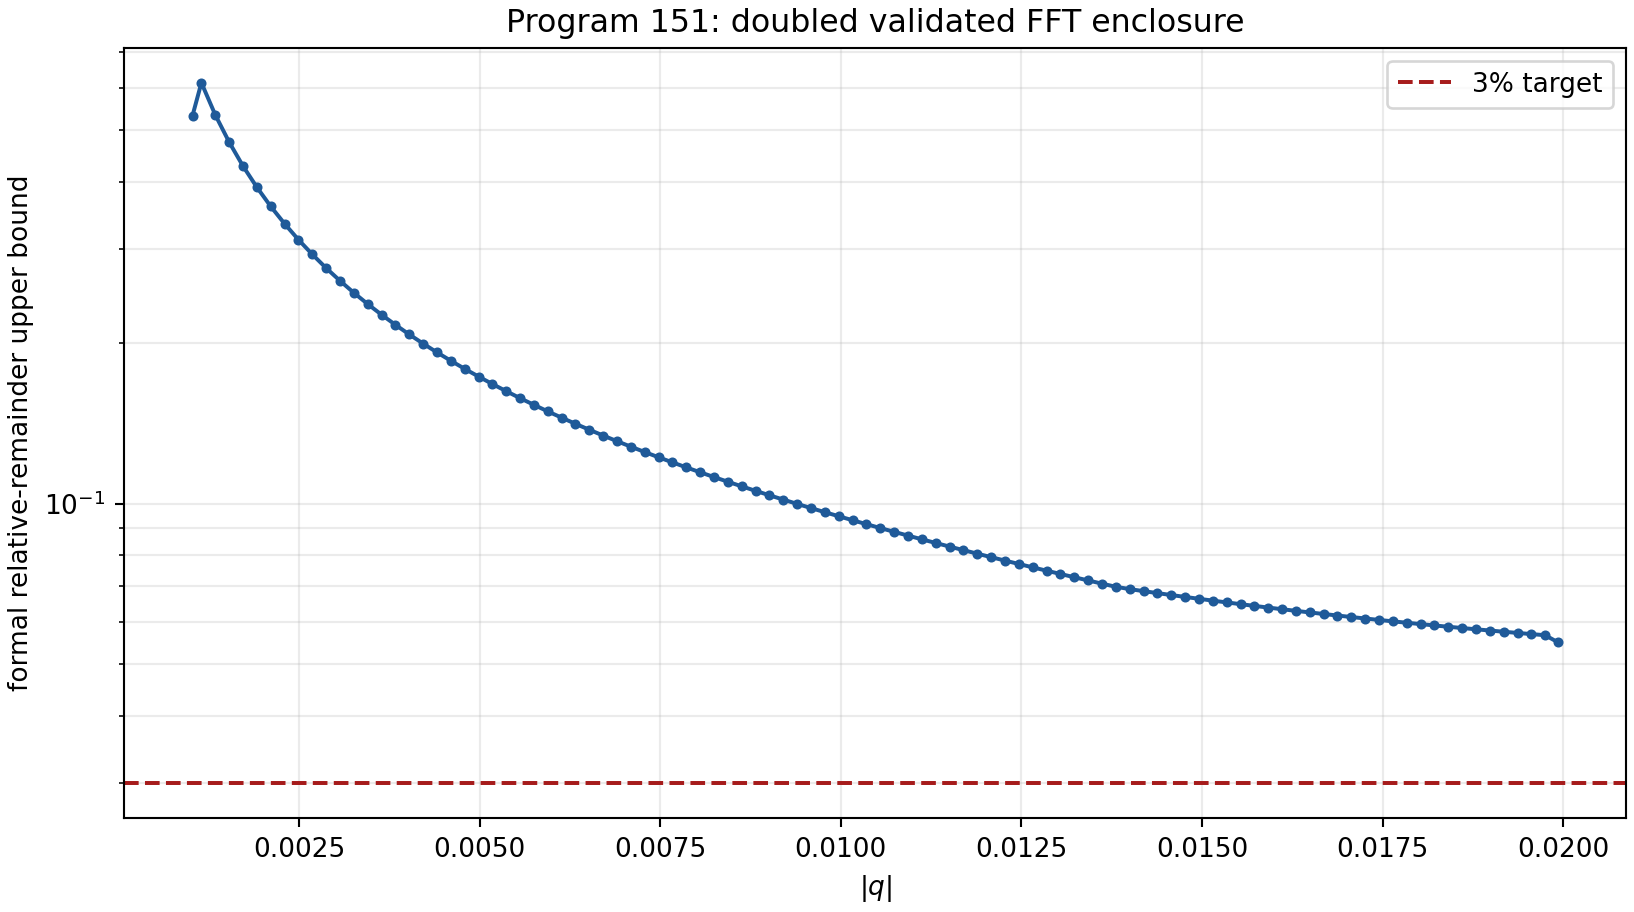
\includegraphics[width=0.94\textwidth]{FIN_Programs_151_164_Axiomatic_Operational_Figures/program151_tighter_interval_fft.png}
\caption{The doubled interval FFT improves the formal enclosure without yet reaching the three-percent target.}
\end{figure}

\section{Interpretation}

The fractional scale is now supported by a stronger theorem, but the tight constant remains open. A future calculation must split the oscillatory tail, use cancellation rather than absolute domination, and preferably use ball-arithmetic FFTs with sharper twiddle enclosures.

\par\medskip\hrule\medskip

\chapter{Program 152 --- The missing Diophantine axiom}

\section{Certified finite arithmetic}

For

\[
\theta=\frac{\omega}{\pi}=\frac{743}{4000\pi},
\]

the first twelve continued-fraction terms remain

\[
[0;16,1,10,2,67,2,2,5,1,2,928].
\]

On this finite convergent prefix,

\[
\min q\|q\theta\|
=0.0010764647999871935,
\]

and

\[
\min q^2\|q\theta\|
=1.486339454993983.
\]

These are finite-prefix constants, not global constants.

\section{Minimal sufficient premise}

The exact extra all-scale premise is:

\[
D(\kappa,\nu):
\qquad
\|q\theta\|\ge\kappa q^{-\nu}
\quad
\text{for every integer }q\ge1,
\]

where \(\kappa>0\) and \(\nu<\infty\).

\textbf{Theorem 152.1 \statusProven{}.} Irrationality of \(\theta\) alone does not imply \(D(\kappa,\nu)\) for any fixed finite \(\nu\).

\textbf{Proof.} A Liouville irrational \(\lambda\) has infinitely many rational approximations satisfying

\[
\left|\lambda-\frac pq\right|<q^{-m}
\]

for arbitrarily large \(m\). Consequently

\[
\|q\lambda\|<q^{1-m}.
\]

For any fixed \(\nu\) and \(\kappa>0\), choose \(m>\nu+1\) and then a sufficiently large Liouville denominator. This gives

\[
\|q\lambda\|<\kappa q^{-\nu},
\]

contradicting \(D(\kappa,\nu)\). \(\square\)

\textbf{Corollary 152.2 \statusProven{}.} No proof using only the proposition "\(\theta\) is irrational" can establish an all-scale polynomial small-divisor bound.

\begin{figure}[htbp]
\centering
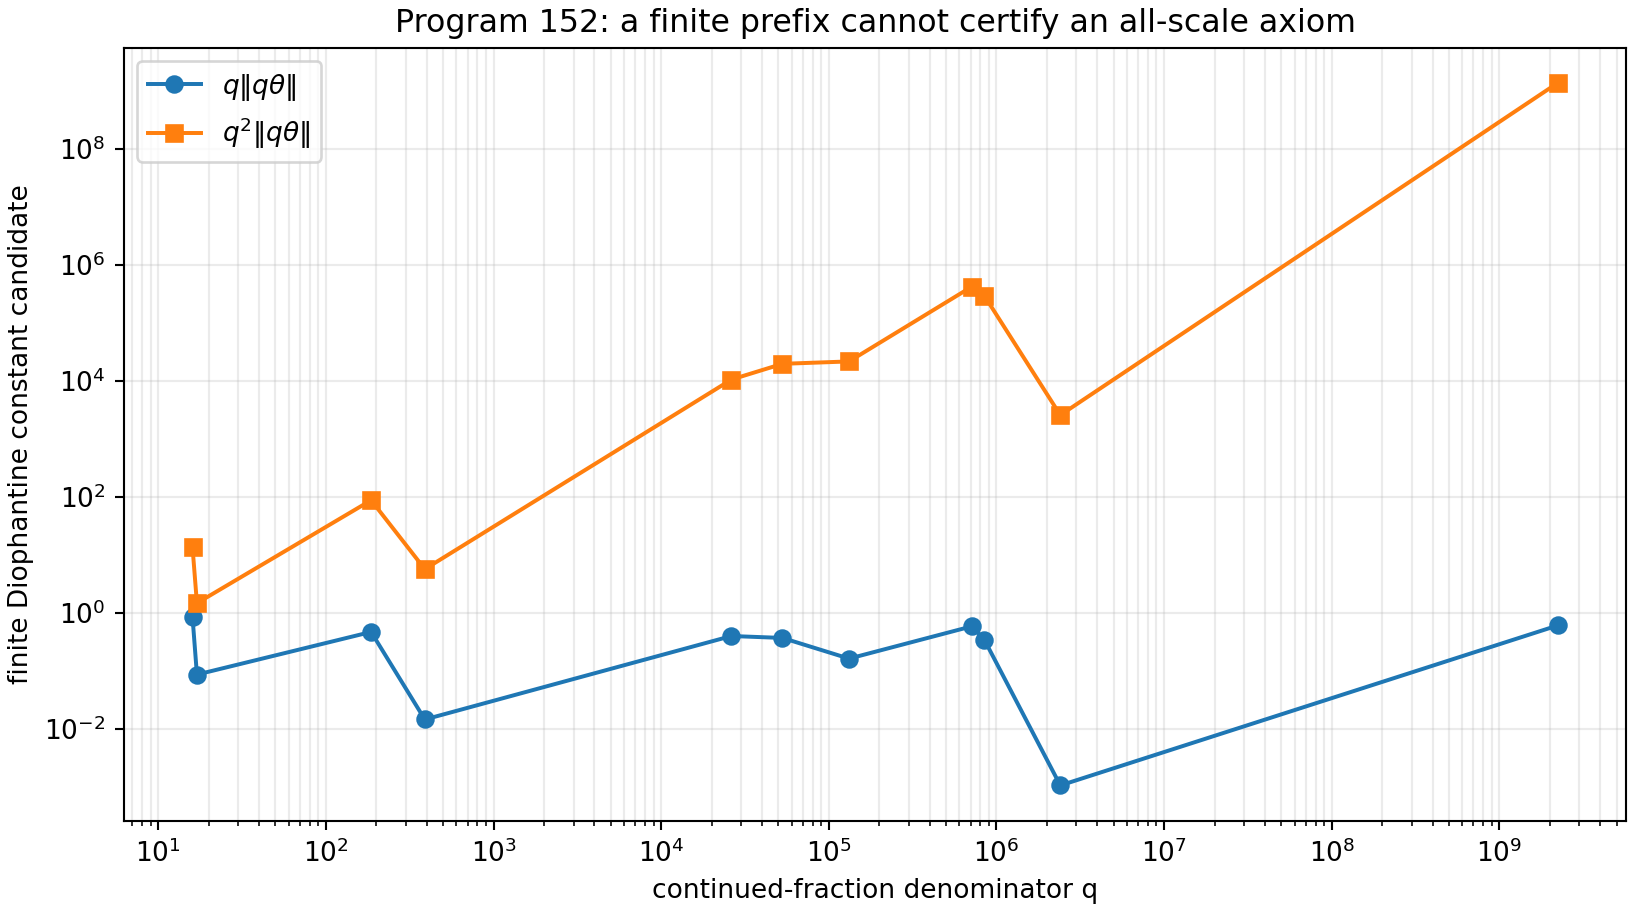
\includegraphics[width=0.94\textwidth]{FIN_Programs_151_164_Axiomatic_Operational_Figures/program152_diophantine_axiom.png}
\caption{Finite candidates for \(q^\nu\lVert q\theta\rVert\) do not certify an all-scale Diophantine axiom.}
\end{figure}

\section{Necessity rank}

The Diophantine axiom has a narrow role. It is not needed to define either \(U_t\) or \(P_t\). It is needed only for a quantitative all-scale rate in the oscillatory Abelian limit. It is therefore a technical regularity axiom, not an axiom of physical ontology.

\par\medskip\hrule\medskip

\chapter{Program 153 --- Functorial fibre-groupoid measures}

\section{Groupoid}

The admitted structural symmetries partition the five localized fibres into three isomorphism orbits:

\[
\{2\},\qquad \{3\},\qquad \{5,7,11\}.
\]

An invariant central state must be constant on each orbit.

\textbf{Theorem 153.1 \statusProven{}.} Every invariant probability measure has the form

\[
(w_2,w_3,w_5,w_7,w_{11})
=(x,y,z/3,z/3,z/3),
\]

where

\[
x,y,z\ge0,\qquad x+y+z=1.
\]

\textbf{Proof.} Invariance forces equality of the three weights in the last orbit. There are no admitted morphisms between distinct orbits, so their total masses remain independent. Normalization removes one of three variables, leaving a two-dimensional simplex. \(\square\)

The uniform sector state corresponds to

\[
(x,y,z)=(1/5,1/5,3/5).
\]

It is one interior point, not a categorical fixed point.

\begin{figure}[htbp]
\centering
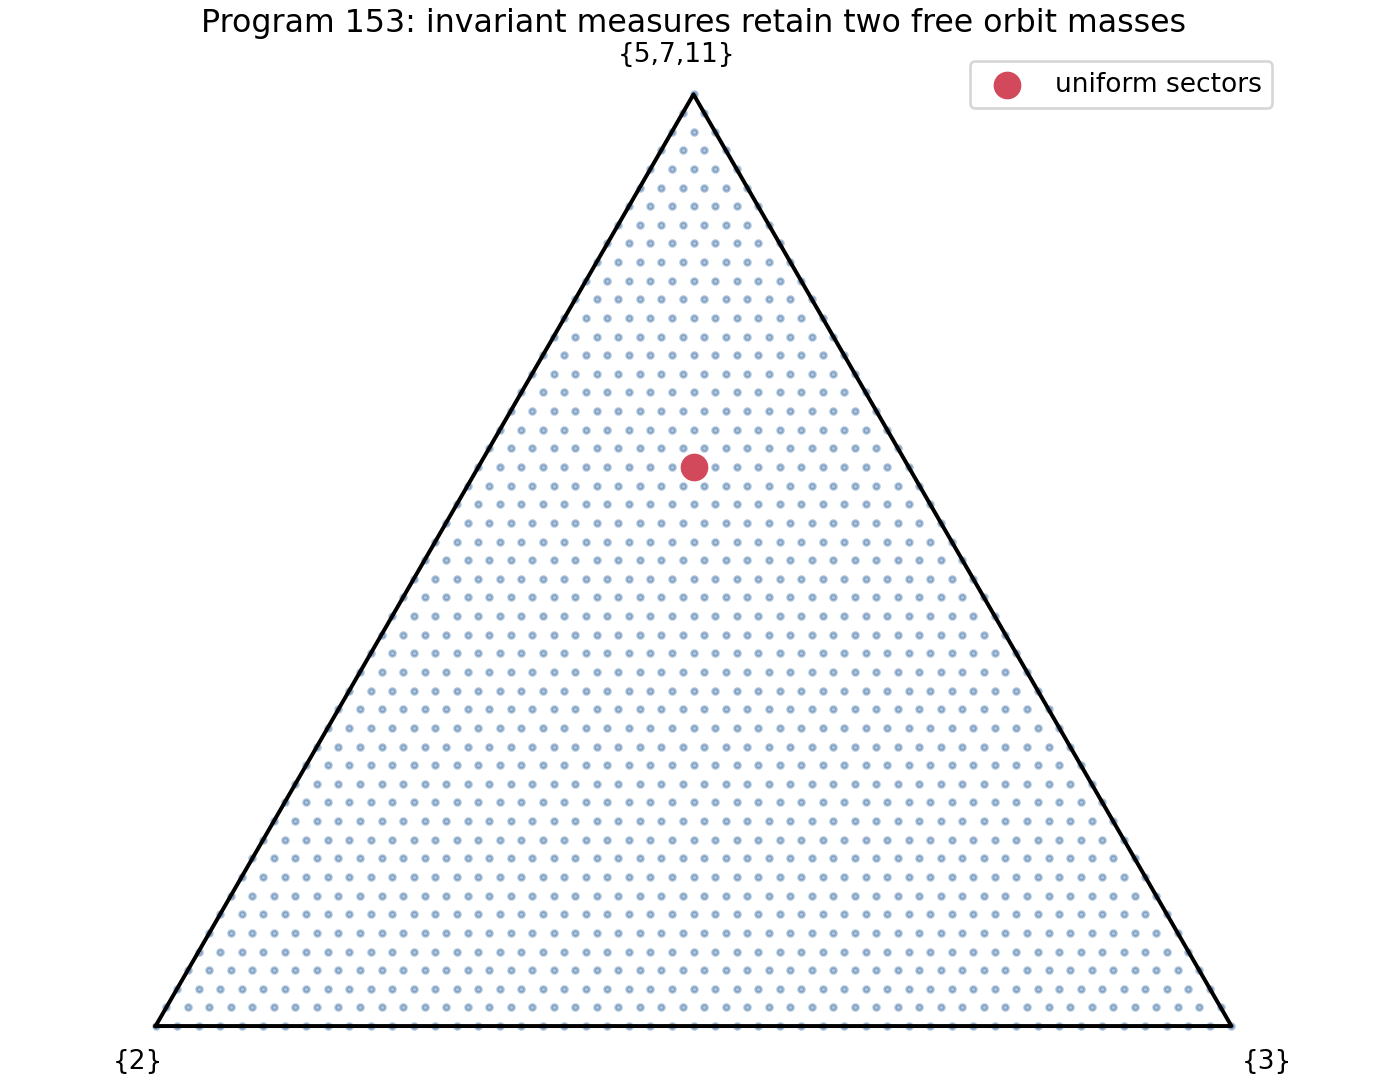
\includegraphics[width=0.94\textwidth]{FIN_Programs_151_164_Axiomatic_Operational_Figures/program153_groupoid_measure_simplex.png}
\caption{Groupoid invariance leaves a two-dimensional simplex of orbit masses.}
\end{figure}

\section{Falsification}

\textbf{Corollary 153.2 \statusRefuted{}.} Normalization, invariance, and additivity do not select \(w_p=1/5\).

An additional monoidal valuation or induction/\allowbreak{}restriction law could reduce the simplex. That law would itself be an added premise and must be tested for uniqueness.

\par\medskip\hrule\medskip

\chapter{Program 154 --- A minimal modular-equilibrium axiom}

\section{Natural carrier energy}

The smallest energy generated by the fibre dimensions is

\[
E_p=d_p-1.
\]

For the Hilbert-block Gibbs state, the central sector mass is

\[
w_p(\beta_F)
=
\frac{d_p e^{-\beta_F E_p}}
{\sum_q d_q e^{-\beta_F E_q}}.
\]

The factor \(d_p\) is the block degeneracy.

\section{The new axiom}

Define

\[
A_{\rm ME}:
\qquad
\beta_F
=
\frac{\alpha_{\rm geo}}
{|\operatorname{Hom}(U(12),\{\pm1\})|}.
\]

Since

\[
|\operatorname{Hom}(U(12),\{\pm1\})|=4,
\qquad
\alpha_{\rm geo}=4\log2,
\]

this becomes

\[
\beta_F=\log2.
\]

\textbf{Theorem 154.1 [Proven conditional on \(A_{\rm ME}\)].} The central Gibbs state is uniform and its dimension expectation is \(9/5\).

\textbf{Proof.} For the one-dimensional fibre,

\[
d_2e^{-\beta_FE_2}=1.
\]

For every two-dimensional fibre,

\[
d_pe^{-\beta_FE_p}
=2e^{-\log2}
=1.
\]

All five unnormalized central masses are equal. Hence \(w_p=1/5\), and

\[
\eta
=
\frac{1+2+2+2+2}{5}
=\frac95.
\]

\(\square\)

\textbf{Theorem 154.2 \statusProven{}.} With Hilbert degeneracy and unit gap, the required positive inverse temperature is unique.

\textbf{Proof.} Equality between a \(d=1\) sector and a \(d=2\) sector requires

\[
1=2e^{-\beta_F}.
\]

Therefore \(\beta_F=\log2\), uniquely. \(\square\)

\begin{figure}[htbp]
\centering
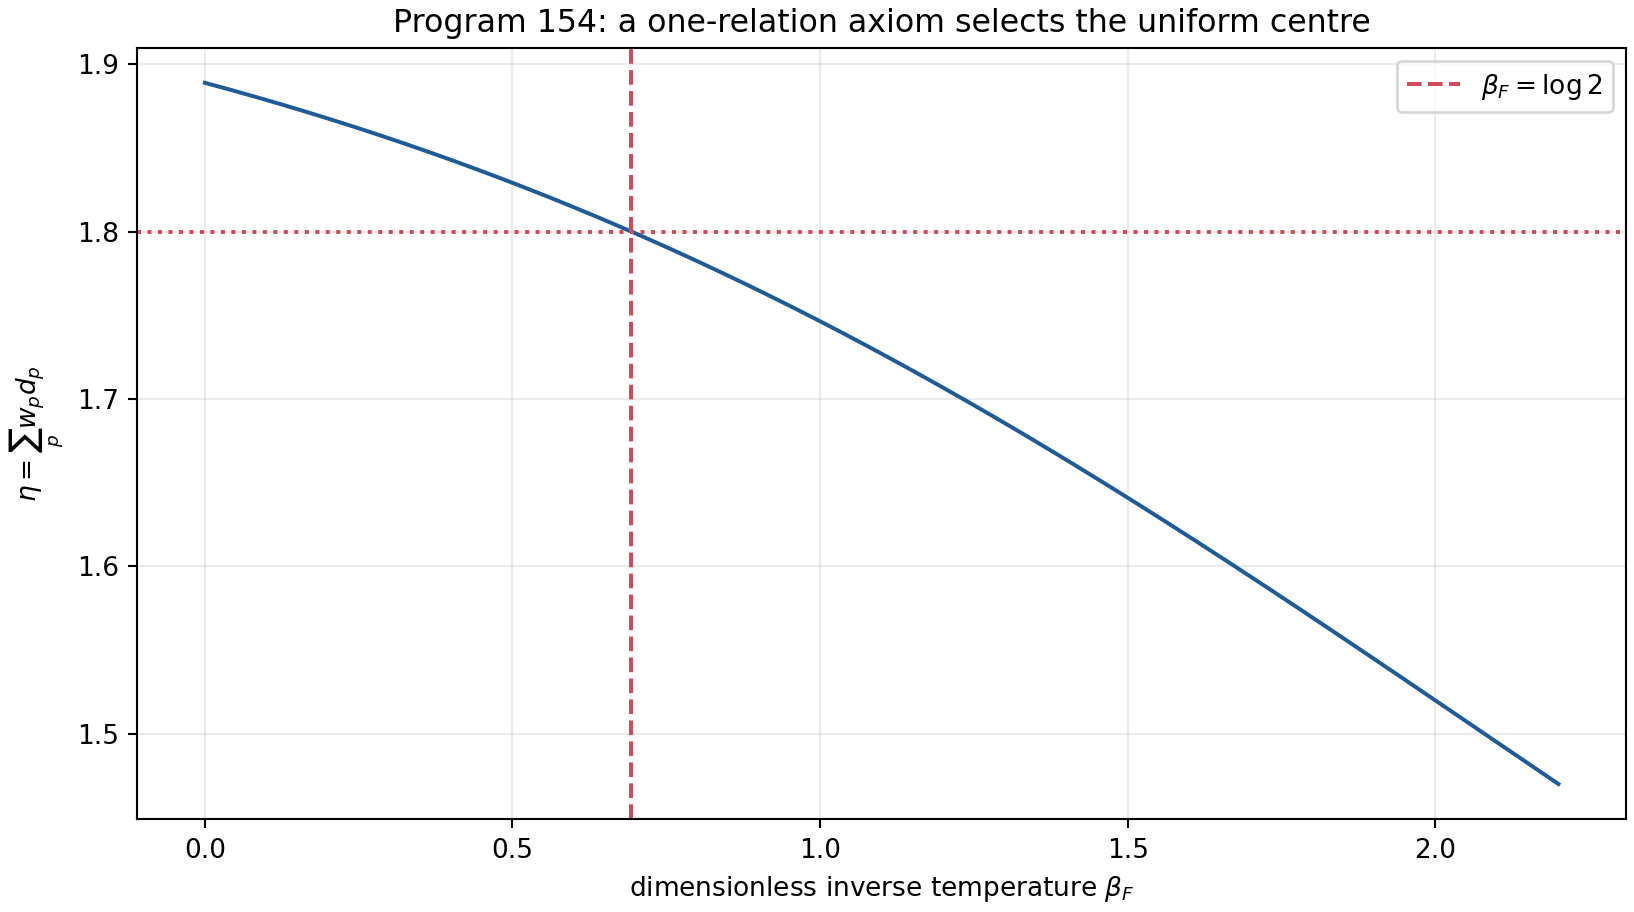
\includegraphics[width=0.94\textwidth]{FIN_Programs_151_164_Axiomatic_Operational_Figures/program154_axiomatic_modular_equilibrium.png}
\caption{The axiom \(\beta_F=\log2\) selects the uniform central state and \(\eta=9/5\).}
\end{figure}

\section{Removal audit}

\begin{center}
\begingroup\small
\setlength{\tabcolsep}{3.5pt}
\renewcommand{\arraystretch}{1.16}
\begin{longtable}{@{}p{0.420\textwidth}p{0.420\textwidth}@{}}
\toprule
\textbf{Removed item} & \textbf{Consequence} \\
\midrule
\endhead
\(A_{\rm ME}\) temperature relation & A continuous Gibbs family remains \\
unit energy gap & only \(\beta_F\Delta=\log2\) is fixed \\
Hilbert degeneracy & sector-counting equilibrium selects uniformity at \(\beta_F=0\) \\
carrier Hamiltonian & no distinguished modular dynamics remains \\
\bottomrule
\end{longtable}
\endgroup
\end{center}

Each ingredient is therefore necessary for this exact construction.

\section{Status}

\(A_{\rm ME}\) is the best single-relation state-selection candidate found in this round. It is scientifically preferable to hiding uniform weights inside a definition because:

\begin{enumerate}
\item 
the new premise is one explicit equation;

\item 
the conclusion is unique;

\item 
every component has a removal test;

\item 
perturbations can be experimentally or mathematically falsified.

\end{enumerate}

It does not fix an orientation, create a nonfree preparation, introduce SI units, or construct the legacy-to-strict phase map.

\par\medskip\hrule\medskip

\chapter{Program 155 --- Completeness of the reflection resource}

Let

\[
\rho_r
=
\frac{1+r}{2}\rho_+
+\frac{1-r}{2}\rho_-,
\qquad -1\le r\le1,
\]

where reflection interchanges \(\rho_+\) and \(\rho_-\).

An affine trace-preserving reflection-covariant map must commute with \(r\mapsto-r\). It therefore has the form

\[
r\longmapsto r'=\lambda r.
\]

Positivity on the whole interval is equivalent to \(|\lambda|\le1\).

\textbf{Theorem 155.1 \statusProven{}.} The monotone

\[
M(\rho_r)=|r|
\]

is complete for deterministic conversion on the reflection orbit line:

\[
\rho_r\longrightarrow\rho_s
\quad\text{by a free channel}
\quad\Longleftrightarrow\quad
|s|\le|r|.
\]

\textbf{Proof.} Necessity follows from \(s=\lambda r\) and \(|\lambda|\le1\). Conversely, if \(r\ne0\) and \(|s|\le|r|\), choose \(\lambda=s/r\). If \(r=0\), only \(s=0\) is allowed. \(\square\)

\begin{figure}[htbp]
\centering
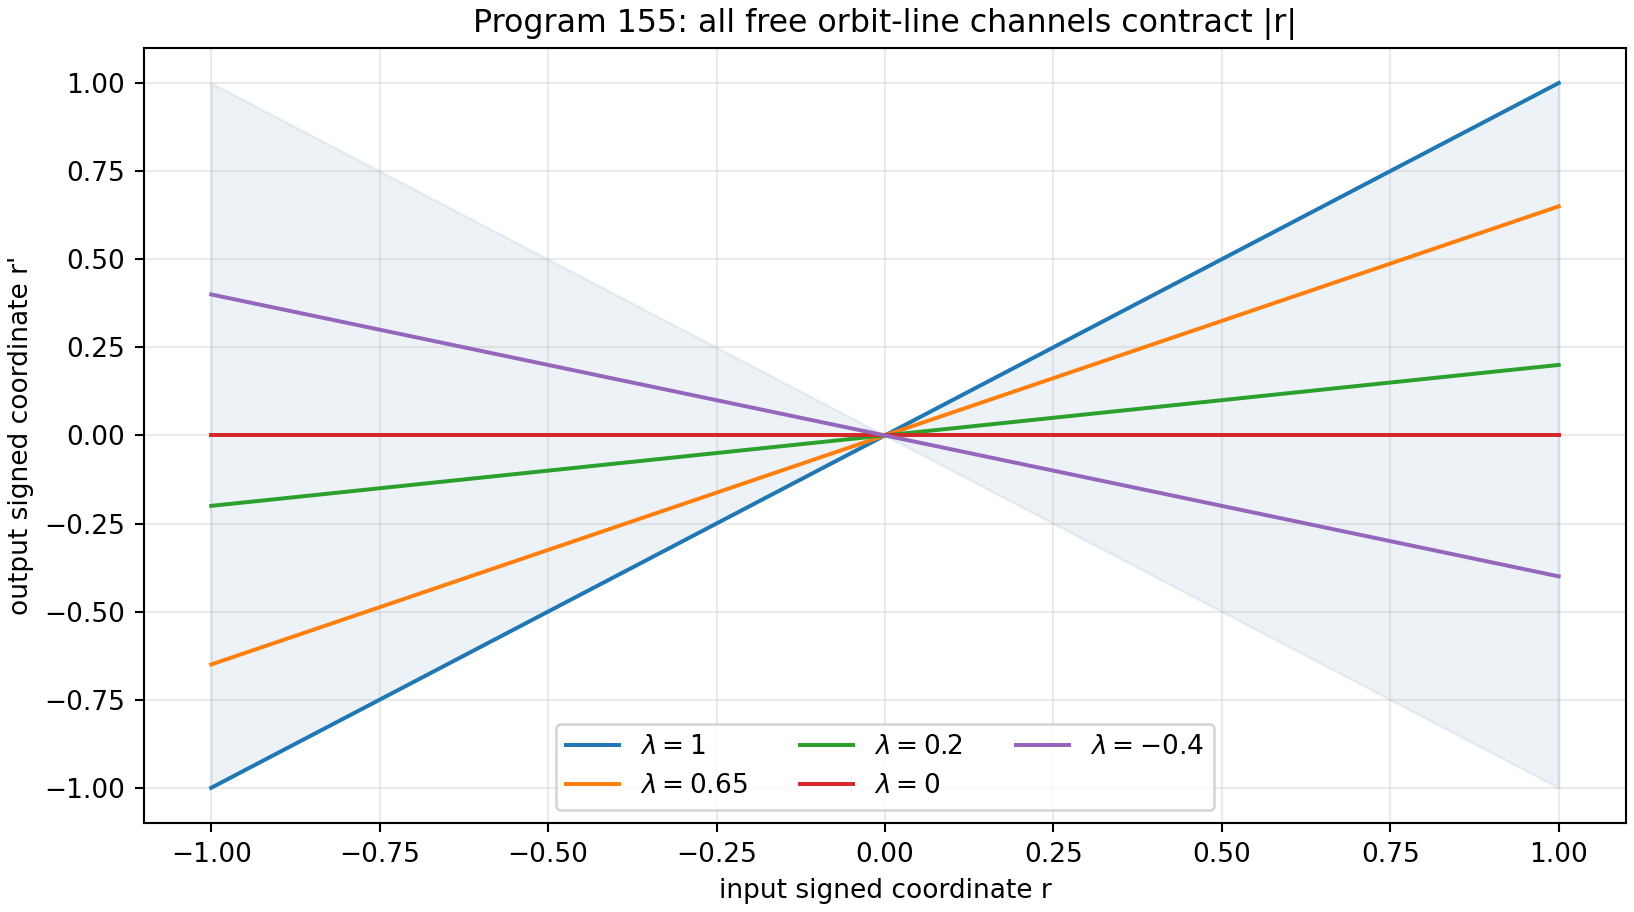
\includegraphics[width=0.94\textwidth]{FIN_Programs_151_164_Axiomatic_Operational_Figures/program155_reflection_resource_complete.png}
\caption{Every reflection-covariant orbit-line channel contracts the complete monotone \(\lvert r\rvert\).}
\end{figure}

This theorem makes the missing signed resource operationally precise. It also strengthens the obstruction: a symmetric preparation is not merely inconvenient; it lies in a distinct resource order and cannot reach a signed state by free processing.

The theorem is restricted to this one-dimensional orbit family. Completeness on the full density-matrix space remains open.

\par\medskip\hrule\medskip

\chapter{Program 156 --- Detector deconvolution and finite bias}

\section{Quartile asymptotics}

For a continuous distribution with density \(f\) positive at its quartiles, the joint empirical-quantile central limit theorem gives

\[
\operatorname{Cov}(\widehat q_p,\widehat q_r)
=
\frac{\min(p,r)-pr}
{n f(q_p)f(q_r)}
+o(n^{-1}).
\]

For a symmetric distribution,

\[
f(q_{0.25})=f(q_{0.75}).
\]

Substitution yields:

\textbf{Theorem 156.1 \statusProven{}.}

\[
\operatorname{Var}(\widehat{\mathrm{IQR}})
=
\frac{1}{4n f(q_{0.75})^2}
+o(n^{-1}).
\]

For independent samples at \(t_1\) and \(t_2\), the delta method gives

\[
\operatorname{Var}(\widehat T)
\sim
\frac{1}{\log^2(t_2/t_1)}
\sum_{j=1}^2
\frac{\operatorname{Var}(\widehat{\mathrm{IQR}}_j)}
{\mathrm{IQR}_j^2}.
\]

For \(\alpha=4/5\), \(n=4000\), and \((t_1,t_2)=(1,4)\), the predicted zero-noise standard deviation is

\[
0.030707238977584036.
\]

\section{Gaussian resolution}

Let the apparatus add an independent Gaussian error with absolute standard deviation \(\sigma\). The simulation used 320 repetitions with 4000 records at each time.

\begin{center}
\begingroup\small
\setlength{\tabcolsep}{3.5pt}
\renewcommand{\arraystretch}{1.16}
\begin{longtable}{@{}p{0.235\textwidth}p{0.190\textwidth}p{0.204\textwidth}p{0.231\textwidth}@{}}
\toprule
\textbf{\(\sigma/\mathrm{IQR}(t_1)\)} & \textbf{mean \(\widehat T\)} & \textbf{bias} & \textbf{standard deviation} \\
\midrule
\endhead
0.00 & 1.248888 & -0.001112 & 0.029793 \\
0.05 & 1.244772 & -0.005228 & 0.029161 \\
0.10 & 1.234645 & -0.015355 & 0.029442 \\
0.20 & 1.190665 & -0.059335 & 0.027095 \\
0.40 & 1.064470 & -0.185530 & 0.027098 \\
\bottomrule
\end{longtable}
\endgroup
\end{center}

\begin{figure}[htbp]
\centering
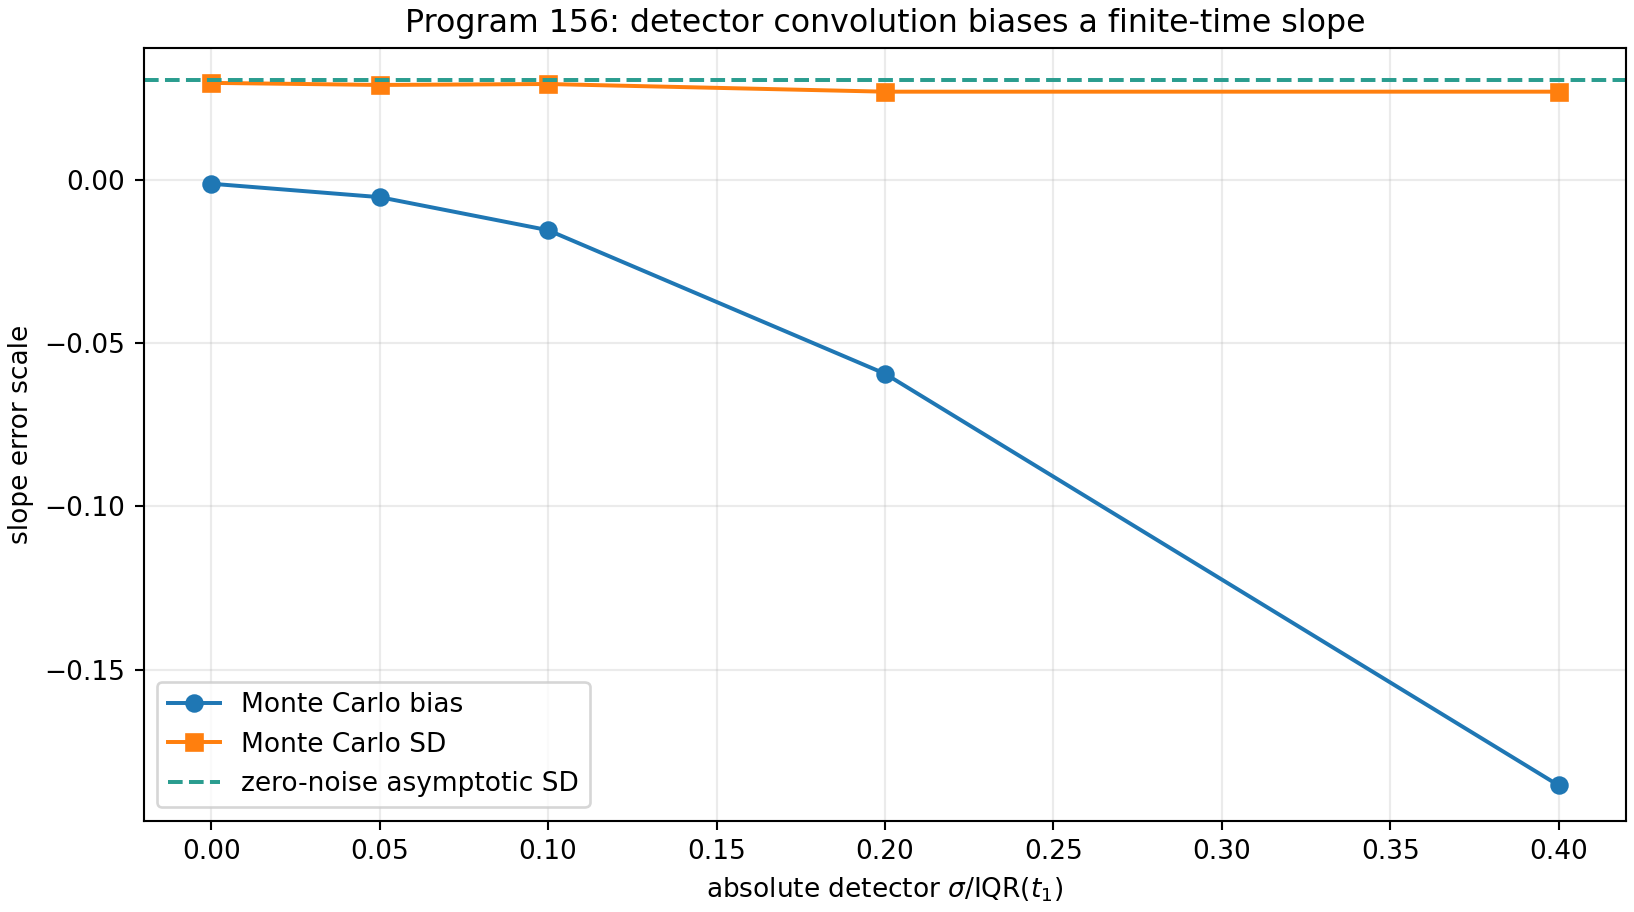
\includegraphics[width=0.94\textwidth]{FIN_Programs_151_164_Axiomatic_Operational_Figures/program156_detector_bias.png}
\caption{Absolute Gaussian resolution biases the finite-time IQR spreading slope downward.}
\end{figure}

\textbf{Result 156.2 \statusStrong{}.} Absolute detector blur reduces the finite time-ratio slope because it is a larger relative perturbation at the earlier, narrower distribution.

\section{Deconvolution theorem boundary}

Gaussian convolution has Fourier multiplier

\[
\widehat R_\sigma(q)=e^{-\sigma^2q^2/2}.
\]

It is never zero, so noiseless deconvolution is algebraically identifiable. Its inverse is

\[
\widehat R_\sigma(q)^{-1}=e^{\sigma^2q^2/2},
\]

which is unbounded. Thus unregularized statistical deconvolution is UV-unstable. Detector calibration does not eliminate the need for a regularization or smoothness class.

\par\medskip\hrule\medskip

\chapter{Program 157 --- Semiparametric system--instrument identifiability}

Suppose a measured scale has the form

\[
Q_{\rm obs}(t)=h(t)C t^{1/\alpha},
\]

where \(h(t)>0\) is an apparatus response.

\textbf{Theorem 157.1 \statusProven{}.} If \(h\) is unrestricted, \(\alpha\) is not identifiable.

\textbf{Proof.} For any alternative \(\alpha'\), define

\[
h'(t)
=
h(t)t^{1/\alpha-1/\alpha'}.
\]

Then

\[
h'(t)Ct^{1/\alpha'}
=
h(t)Ct^{1/\alpha}
=Q_{\rm obs}(t).
\]

The full record is identical for all \(\alpha'\). \(\square\)

\section{Tangent-space test}

Write \(x=\log t\). The exponent score is proportional to \(x\). If

\[
\log h(t)=\gamma_0+\gamma_1x+\cdots+\gamma_rx^r,
\]

then:

\begin{itemize}
\item 
for \(r=0\), the exponent score is independent of the nuisance tangent;

\item 
for every \(r\ge1\), the score lies exactly in the nuisance tangent space.

\end{itemize}

The seven-time numerical design gives residual norm \(4.77577\) for a constant gain and \(3.05\times10^{-15}\) once a linear gain term is admitted.

\begin{figure}[htbp]
\centering
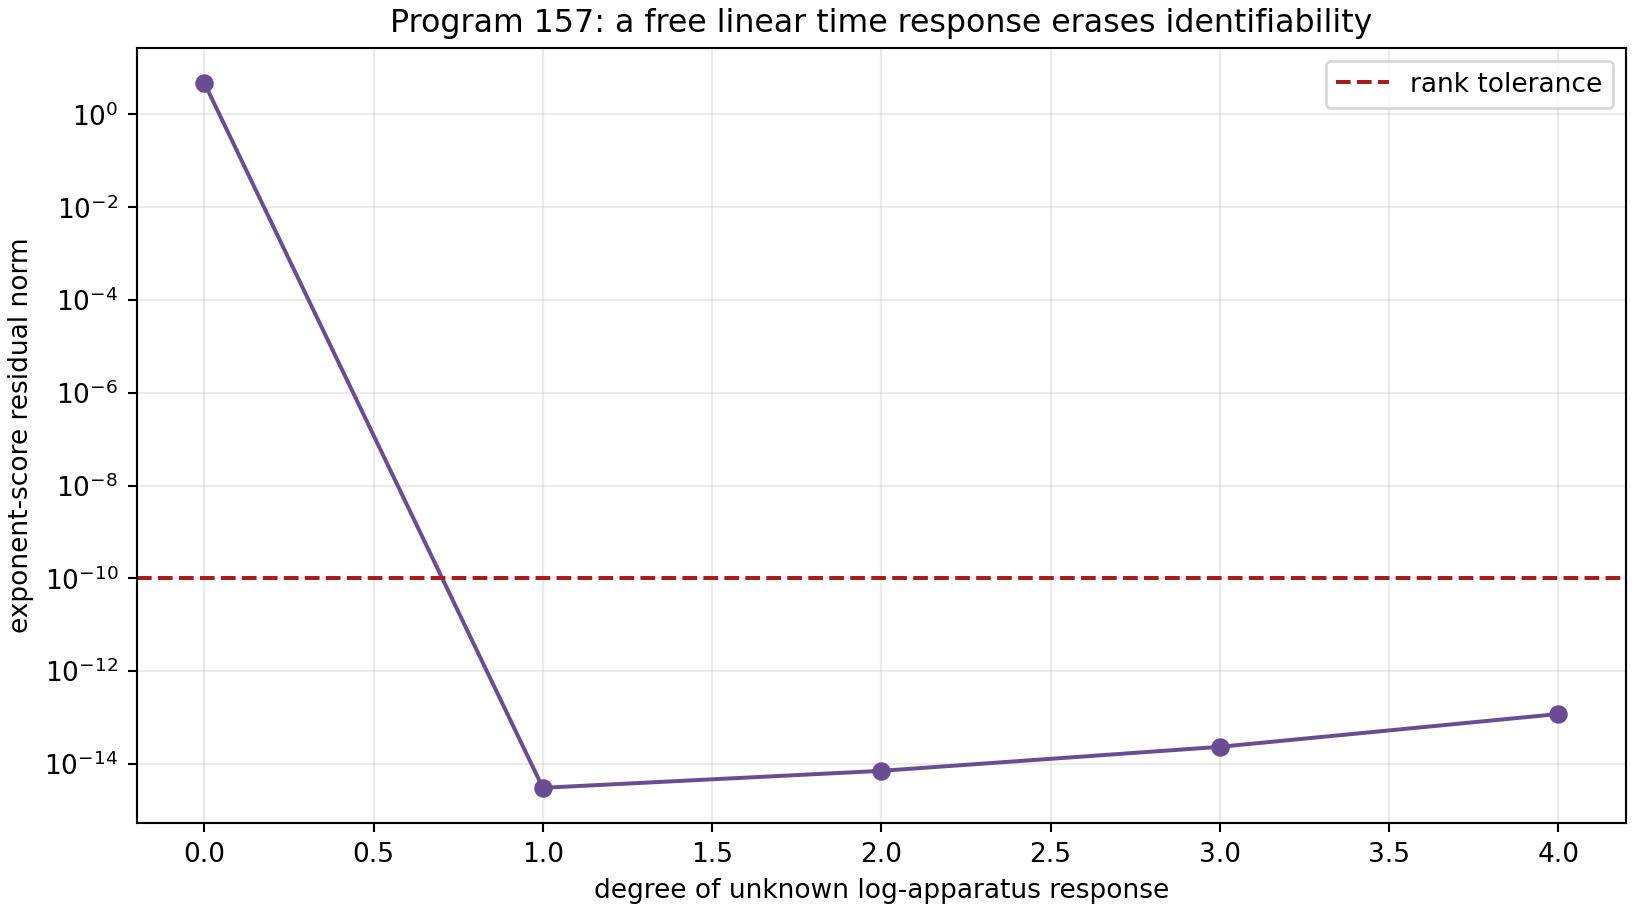
\includegraphics[width=0.94\textwidth]{FIN_Programs_151_164_Axiomatic_Operational_Figures/program157_semiparametric_rank.png}
\caption{A linear log-time apparatus response exactly confounds the fractional exponent.}
\end{figure}

\textbf{Corollary 157.2 \statusProven{}.} More time points do not solve the problem if the apparatus family contains the same log-time direction as the physical exponent. Identification requires external calibration, control preparations, or an independently justified restriction on \(h\).

This is the sharpest operational obstruction of the round.

\par\medskip\hrule\medskip

\chapter{Program 158 --- Finite-sample stable-IQR inference}

For the symmetric \(\alpha=4/5\) stable model, 700 independent repetitions were computed at four sample sizes.

\begin{center}
\begingroup\footnotesize
\setlength{\tabcolsep}{3.5pt}
\renewcommand{\arraystretch}{1.16}
\begin{longtable}{@{}p{0.105\textwidth}p{0.177\textwidth}p{0.198\textwidth}p{0.198\textwidth}p{0.182\textwidth}@{}}
\toprule
\textbf{\(n\)} & \textbf{mean \(\widehat T\)} & \textbf{empirical SD} & \textbf{predicted SD} & \textbf{95\% coverage} \\
\midrule
\endhead
250 & 1.255019 & 0.122981 & 0.122829 & 0.9500 \\
500 & 1.258670 & 0.087482 & 0.086853 & 0.9500 \\
1000 & 1.249667 & 0.063815 & 0.061414 & 0.9414 \\
4000 & 1.248565 & 0.029426 & 0.030707 & 0.9500 \\
\bottomrule
\end{longtable}
\endgroup
\end{center}

\begin{figure}[htbp]
\centering
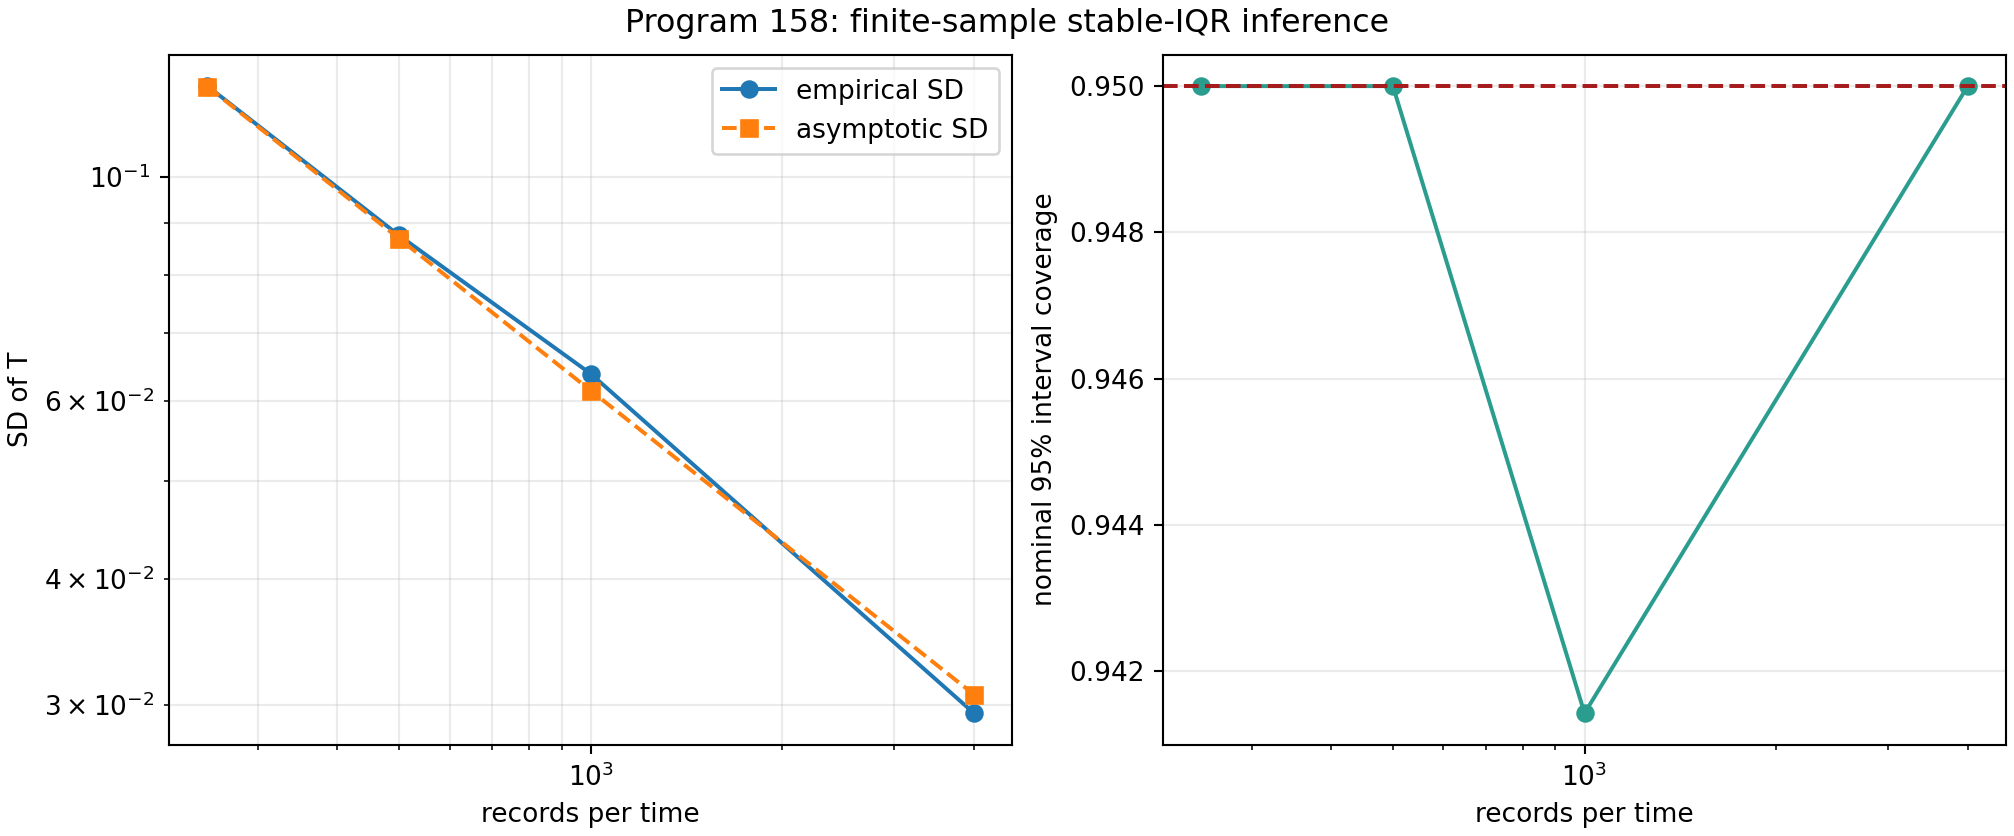
\includegraphics[width=0.94\textwidth]{FIN_Programs_151_164_Axiomatic_Operational_Figures/program158_iqr_finite_sample.png}
\caption{Empirical IQR-slope uncertainty agrees with the asymptotic quantile theorem.}
\end{figure}

\textbf{Result 158.1 \statusStrong{}.} The first-order asymptotic variance is already accurate at \(n=250\) in the declared stable model. The nominal interval has coverage between \(0.941\) and \(0.950\) in the audited range.

\textbf{Boundary.} This is not a distribution-free nonasymptotic theorem. Detector memory, censoring, pixelization, and estimated response parameters can change coverage.

\par\medskip\hrule\medskip

\chapter{Program 159 --- Adversarial protocol challenge}

The Program-150 rule was kept fixed:

\[
\text{declare fractional rather than local diffusion if }
\widehat T>0.875.
\]

Six hidden synthetic families were then generated.

\begin{center}
\begingroup\small
\setlength{\tabcolsep}{3.5pt}
\renewcommand{\arraystretch}{1.16}
\begin{longtable}{@{}p{0.335\textwidth}p{0.143\textwidth}p{0.161\textwidth}p{0.221\textwidth}@{}}
\toprule
\textbf{family} & \textbf{mean \(T\)} & \textbf{P150 decision rate} & \textbf{exploratory FIN-band rate} \\
\midrule
\endhead
local Gaussian & 0.500667 & 0.0000 & 0.0000 \\
stable \(\alpha=0.8\) & 1.251819 & 1.0000 & 1.0000 \\
stable \(\alpha=1.0\) & 0.999638 & 1.0000 & 0.0000 \\
stable \(\alpha=1.2\) & 0.832088 & 0.0656 & 0.0000 \\
absolute-truncated \(\alpha=0.8\) & 1.247964 & 1.0000 & 1.0000 \\
local Gaussian plus time gain & 1.200230 & 1.0000 & 1.0000 \\
\bottomrule
\end{longtable}
\endgroup
\end{center}

The exploratory FIN band was \(1.10\le T\le1.40\) and was not part of the original rule.

\begin{figure}[htbp]
\centering
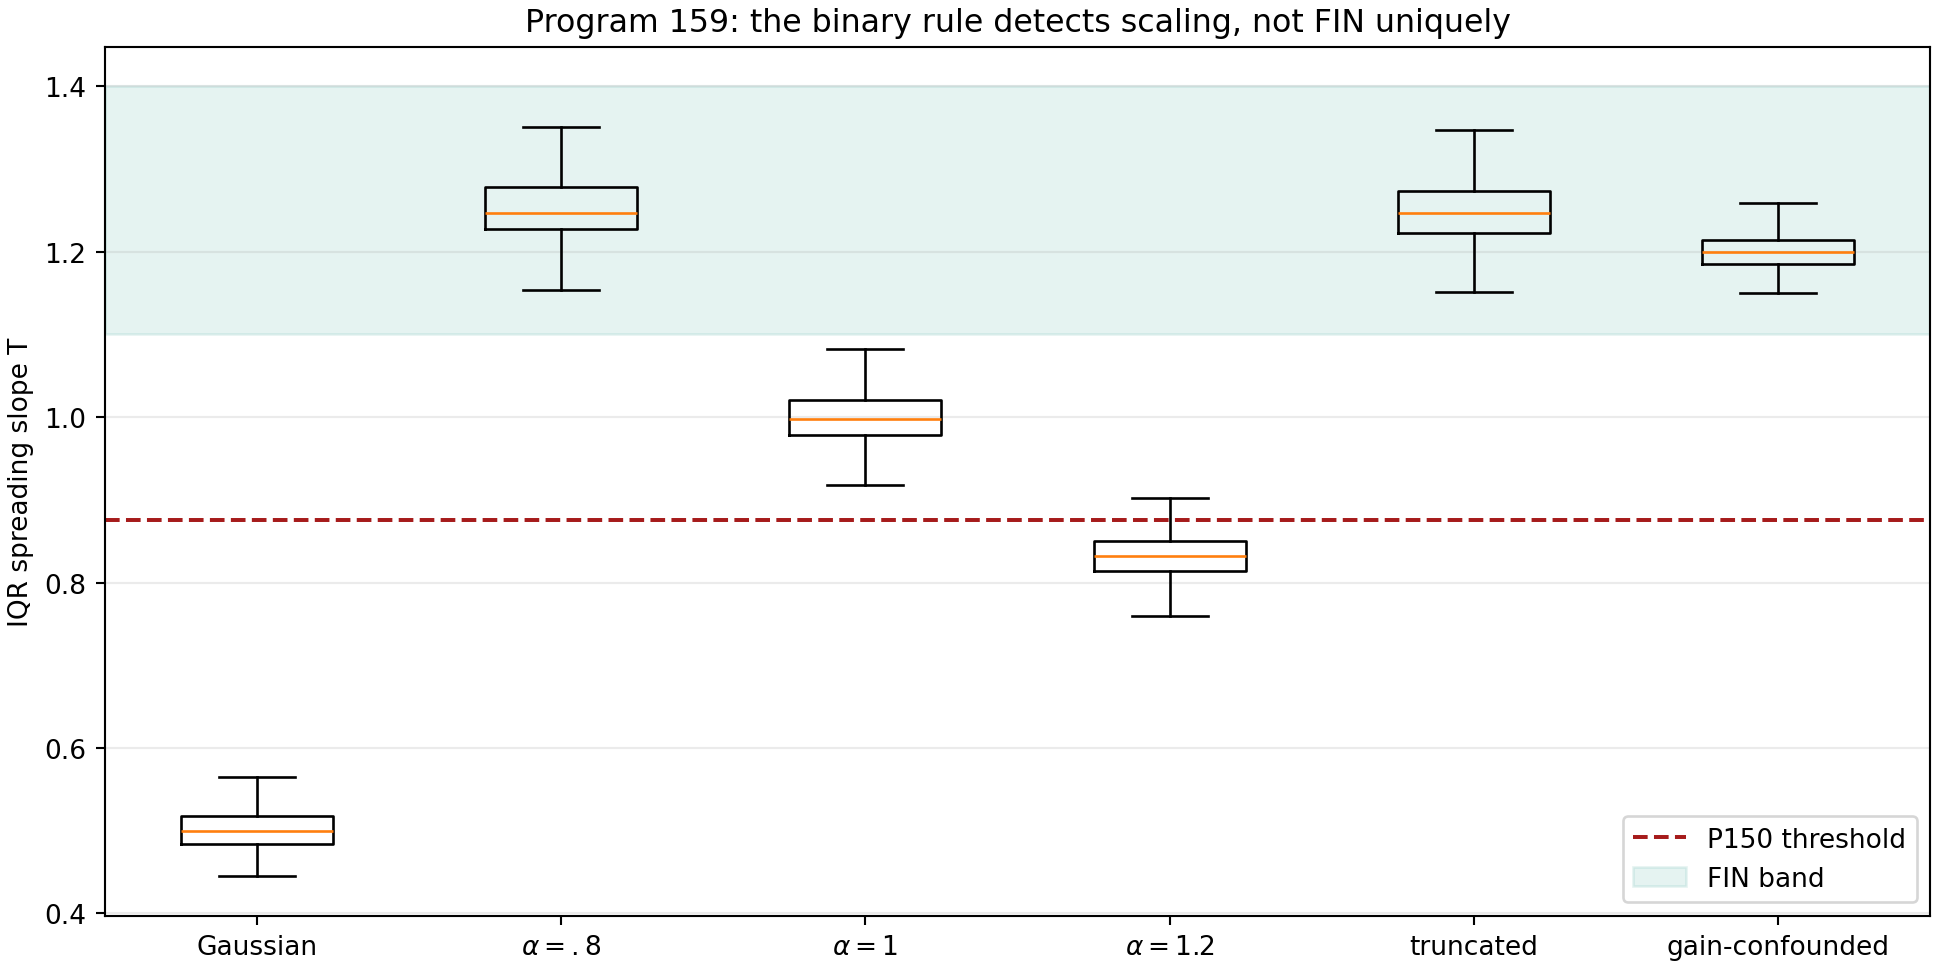
\includegraphics[width=0.94\textwidth]{FIN_Programs_151_164_Axiomatic_Operational_Figures/program159_adversarial_protocol.png}
\caption{The frozen binary rule detects scaling but is not specific to FIN.}
\end{figure}

\section{Falsification}

\textbf{Result 159.1 \statusStrong{}.} The frozen threshold is a good local-versus-fast-spreading discriminator in the declared families, but it is not FIN-specific.

Two counterexamples are decisive:

\begin{enumerate}
\item 
an \(\alpha=1\) stable process is accepted with probability one by the binary threshold;

\item 
a locally diffusive process multiplied by an uncalibrated gain \(t^{0.7}\) enters even the narrower FIN band.

\end{enumerate}

The absolute tail truncation is also invisible to the IQR at the audited cutoff because the central quartiles remain inside the truncation region. Thus IQR robustness is simultaneously a strength and a loss of tail-model specificity.

\textbf{Conclusion.} A successful IQR experiment can estimate a scaling exponent. It cannot by itself prove the FIN kernel, its ontology, or its completion map.

\par\medskip\hrule\medskip

\chapter{Program 160 --- Phase/\allowbreak{}frequency bridge obstruction}

The legacy oscillatory character is

\[
\chi_L(d)=e^{i\pi d/4}.
\]

It is a character of \(\mathbb Z_8\) and has exact order eight.

The strict oscillatory sequence is

\[
\chi_S(d)=e^{i(743/4000)d}.
\]

\textbf{Theorem 160.1 \statusProven{}.} \(\chi_S(1)\) has infinite order.

\textbf{Proof.} If \(\chi_S(1)^T=1\) for an integer \(T>0\), then

\[
\frac{743}{4000}T=2\pi k
\]

for an integer \(k\). The case \(k=0\) is impossible. For \(k\ne0\), this equation makes \(\pi\) rational, a contradiction. \(\square\)

The \(\mathbb Z_{12}\) character defect is

\[
|e^{i12(743/4000)}-1|
=1.7953811736364134.
\]

The generator eigenvalue mismatch is

\[
|e^{i\pi/4}-e^{i743/4000}|
=0.5907042818342478.
\]

\textbf{Theorem 160.2 \statusProven{}.} There is no translation-equivariant character homomorphism from the legacy period-eight representation to the strict infinite-order representation that preserves the generator eigenvalue.

\textbf{Proof.} A homomorphism maps an element of finite order to an element whose order divides that finite order. The proposed image has infinite order. \(\square\)

\begin{figure}[htbp]
\centering
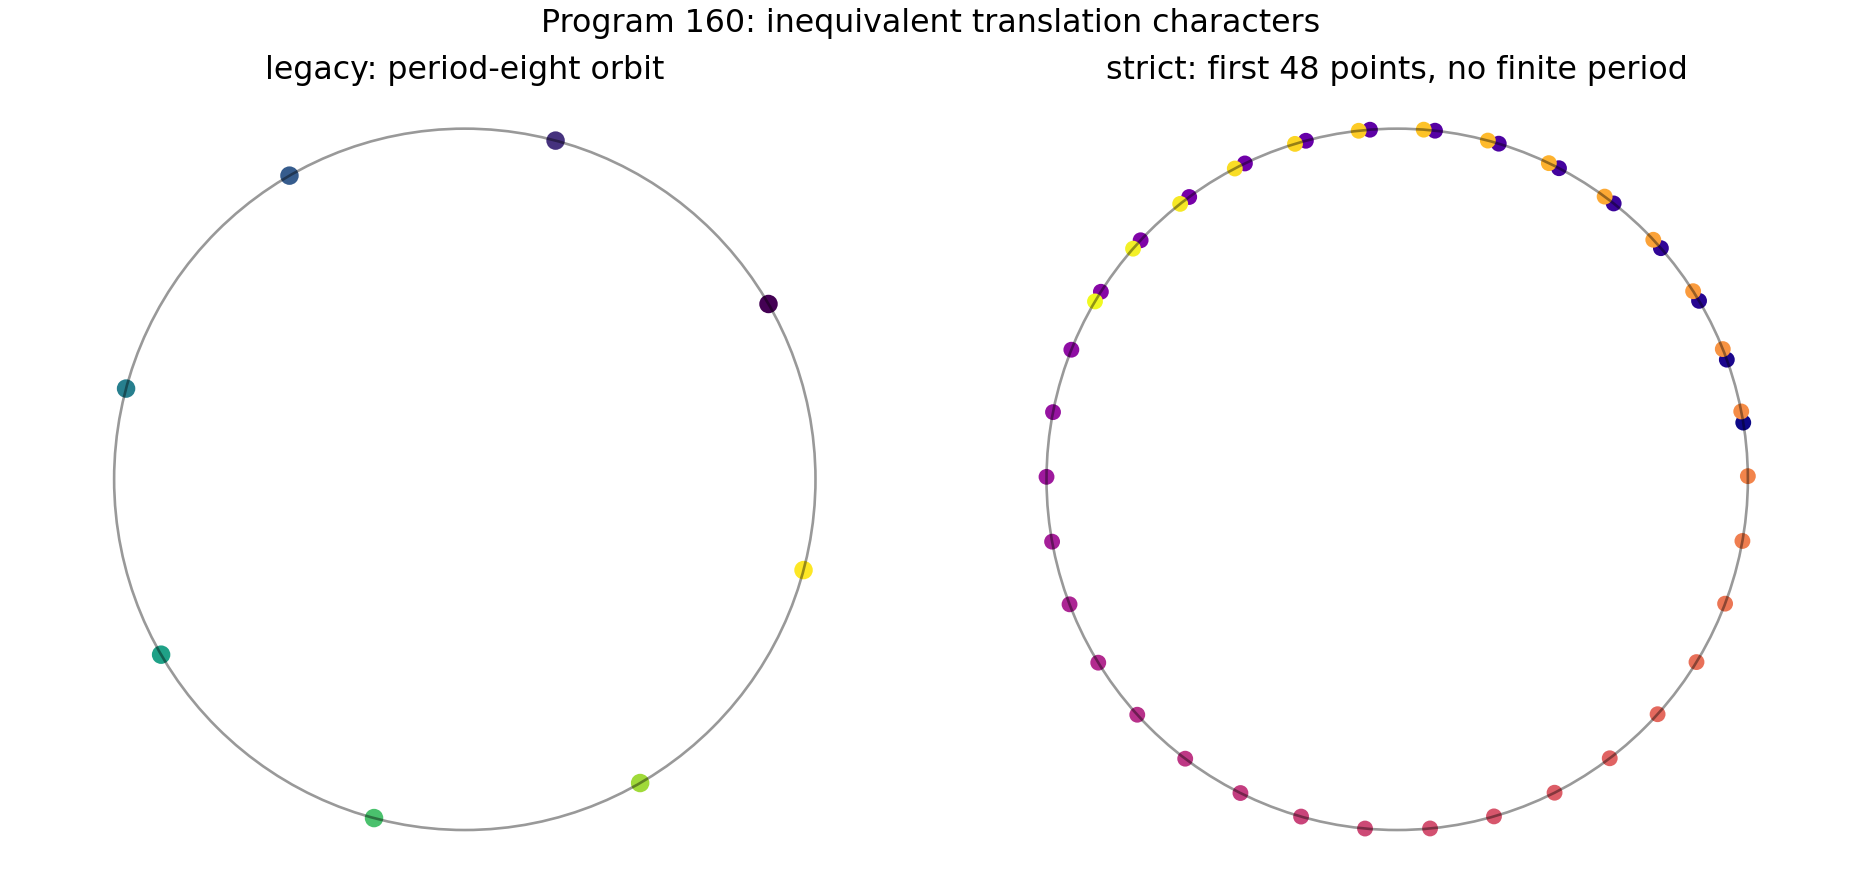
\includegraphics[width=0.94\textwidth]{FIN_Programs_151_164_Axiomatic_Operational_Figures/program160_phase_obstruction.png}
\caption{The period-eight legacy character and infinite-order strict phase are representation-theoretically distinct.}
\end{figure}

This theorem does not exclude a nonlinear or explicitly symmetry-breaking completion. It proves that such a completion cannot be a silent identification of the two translation characters.

\par\medskip\hrule\medskip

\chapter{Program 161 --- Reference-energy grammar}

\section{Declared grammar}

Three orbit-invariant feature columns were used:

\[
f_d=(0,1,1,1,1),
\]

\[
f_3=(0,1,0,0,0),
\]

and

\[
f_U=(0,0,1,1,1).
\]

The energy grammar is

\[
E=c_df_d+c_3f_3+c_Uf_U,
\qquad c_d,c_3,c_U\in\{-3,\ldots,3\}.
\]

All \(7^3=343\) formulas were enumerated. Additive constants are irrelevant.

\textbf{Theorem 161.1 [Proven, exhaustive in the declared grammar].} Six formulas produce the target normalized energy \((0,1,1,1,1)\). The unique minimum \(\ell^1\)-complexity formula is

\[
(c_d,c_3,c_U)=(1,0,0),
\]

that is,

\[
E=d-1.
\]

\begin{figure}[htbp]
\centering
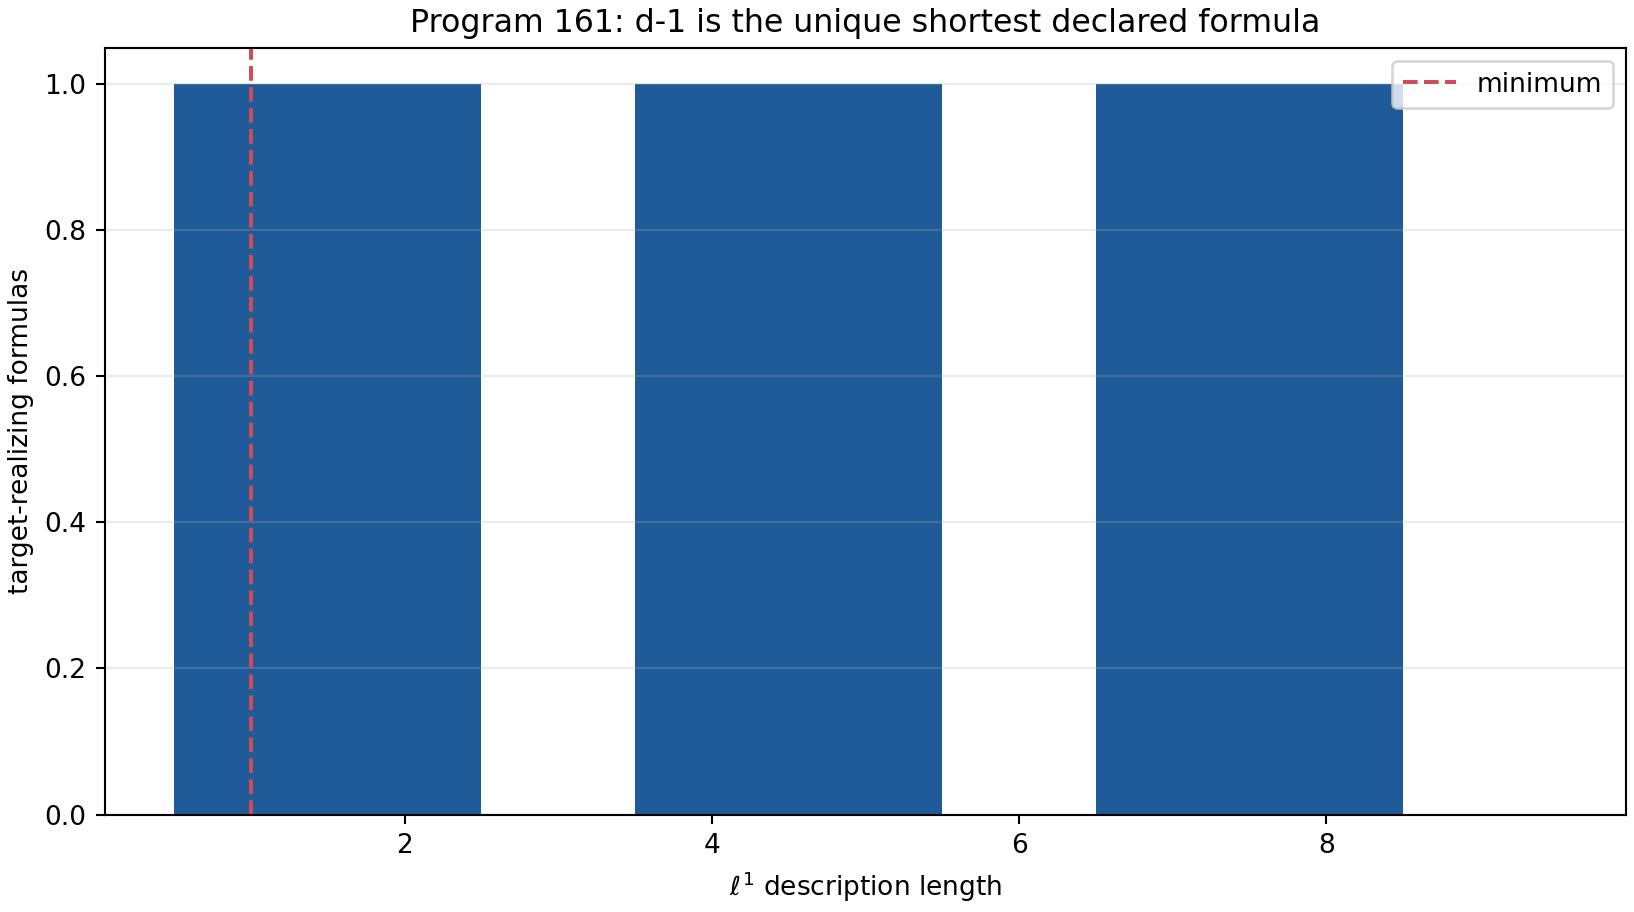
\includegraphics[width=0.94\textwidth]{FIN_Programs_151_164_Axiomatic_Operational_Figures/program161_energy_grammar.png}
\caption{The energy \(d-1\) is the unique shortest target-realizing formula in the declared grammar.}
\end{figure}

The result explains why \(d-1\) is a reasonable carrier Hamiltonian: it is the shortest formula in a transparent structural grammar. It does not prove the target uniform state or the inverse temperature. Minimum description length is relative to its grammar.

\par\medskip\hrule\medskip

\chapter{Program 162 --- Conditional role-transfer obstruction matrix}

A future completion map must address six independent edges:

\begin{enumerate}
\item 
amplitude and normalization;

\item 
damping/\allowbreak{}compression semantics;

\item 
phase and frequency;

\item 
selector and topology;

\item 
physical dimensions and units;

\item 
spectral equivalence at the required operator level.

\end{enumerate}

Nine legacy roles were mapped to their necessary edges.

\begin{figure}[htbp]
\centering
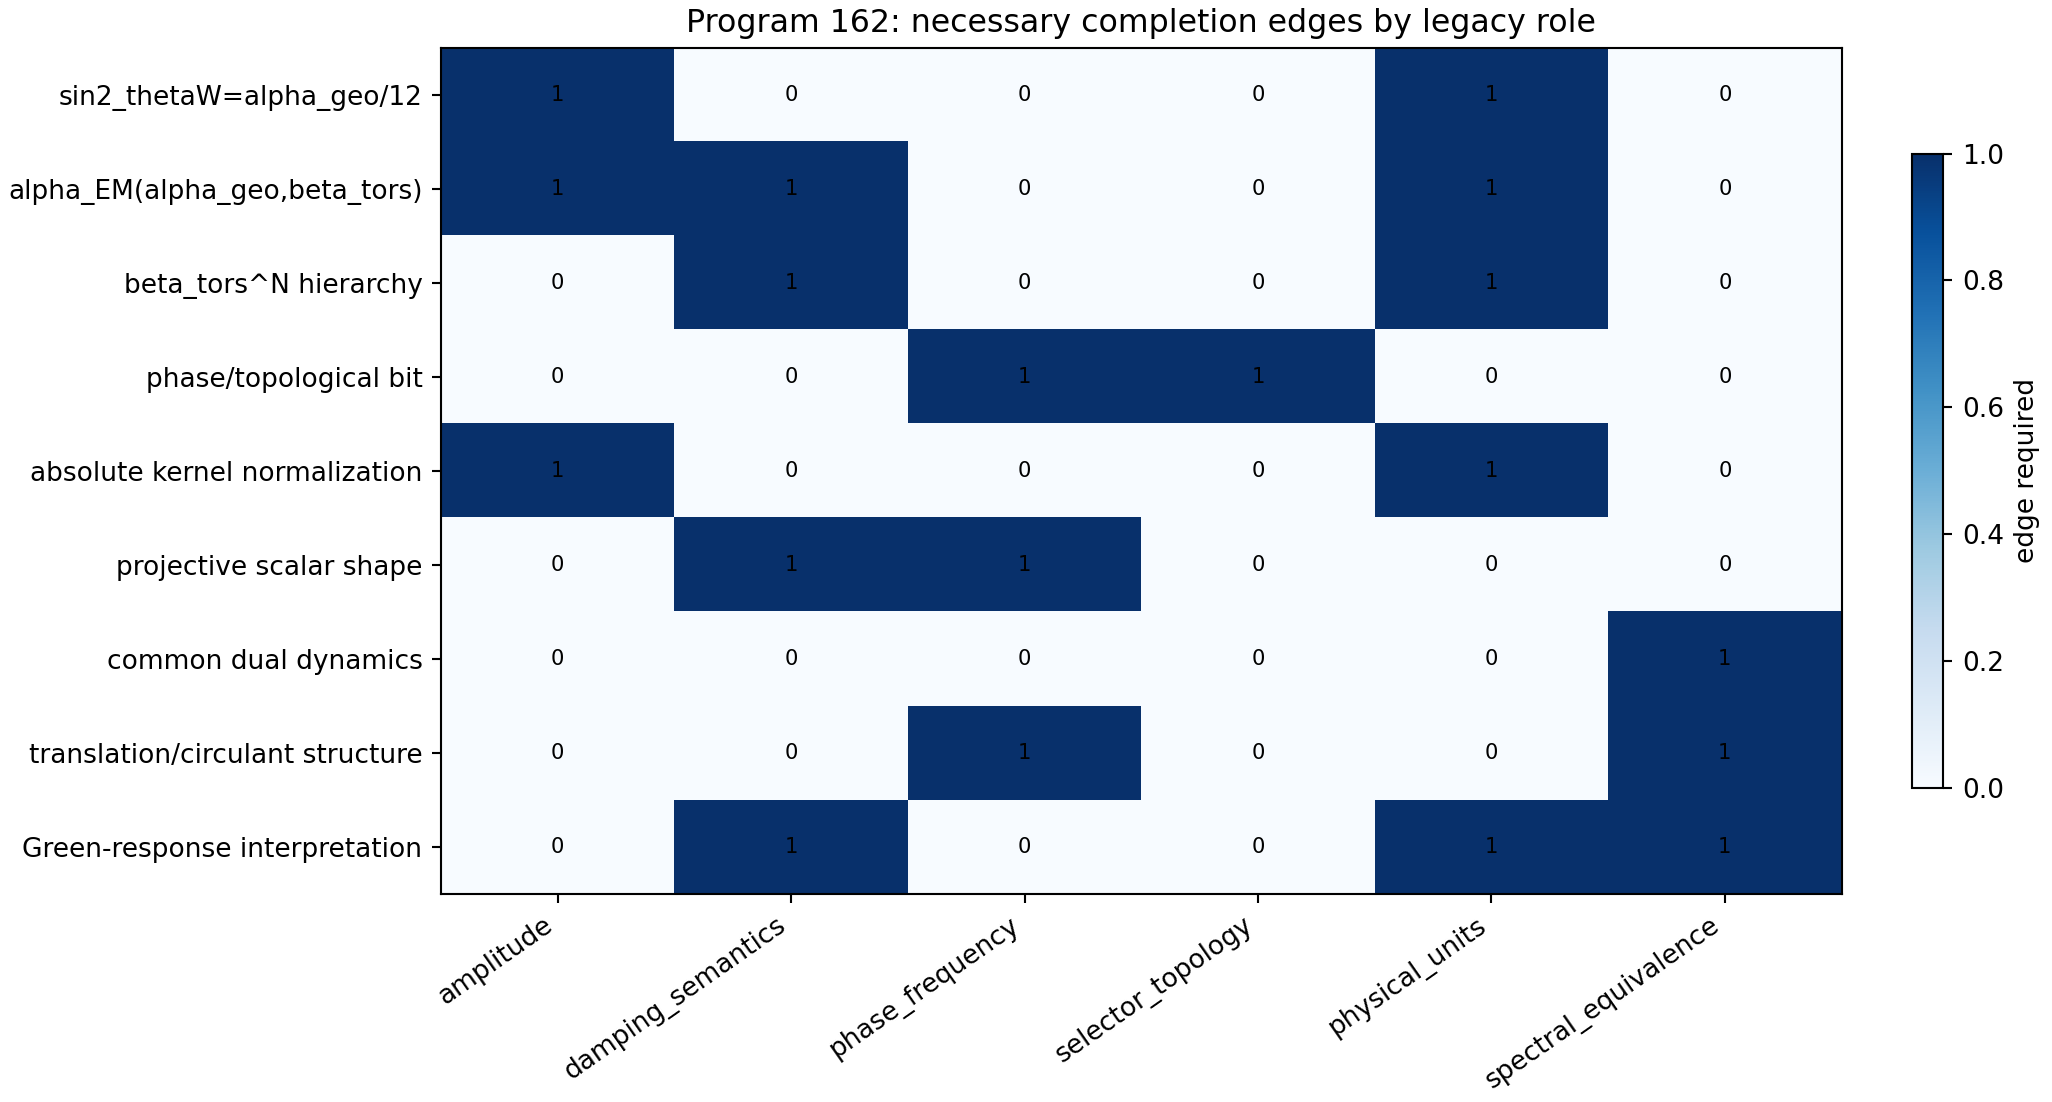
\includegraphics[width=0.94\textwidth]{FIN_Programs_151_164_Axiomatic_Operational_Figures/program162_role_obstruction_matrix.png}
\caption{Necessary completion edges for nine legacy roles; none currently licenses transfer.}
\end{figure}

\section{Result}

\textbf{Theorem 162.1 [Proven in the declared dependency model].} With no complete edge currently exported, zero of the following roles is eligible for transfer:

\begin{itemize}
\item 
\(\sin^2\theta_W=\alpha_{\rm geo}/12\);

\item 
the \(\alpha_{\rm EM}(\alpha_{\rm geo},\beta_{\rm tors})\) formula;

\item 
the \(\beta_{\rm tors}^N\) hierarchy;

\item 
phase/\allowbreak{}topological-bit semantics;

\item 
absolute kernel normalization;

\item 
projective scalar shape as a full bridge claim;

\item 
common dual dynamics as spectral equivalence;

\item 
translation/\allowbreak{}circulant structure as a transported role;

\item 
a dimensional Green-response interpretation.

\end{itemize}

Both kernels can separately generate operator dynamics after suitable positivity shifts. This is a structural analogy, not a proof of spectral equivalence.

The role audit therefore remains downstream. It may begin only after a typed completion map supplies the missing edge appropriate to each role.

\par\medskip\hrule\medskip

\chapter{Program 163 --- External intake readiness}

The immutable protocol

\[
\texttt{FIN-P150-FRACTIONAL-IQR-001}
\]

was reused without altering its core hash. Its mandatory raw-record fields are:

\begin{itemize}
\item 
record identifier;

\item 
preparation batch;

\item 
time;

\item 
position readout;

\item 
detector calibration identifier;

\item 
timestamp.

\end{itemize}

The intake validator accepts JSON or CSV candidates only if these mandatory fields exist. Further gates require two declared times, at least 4000 records per time, detector resolution, memory calibration, and provenance.

\begin{figure}[htbp]
\centering
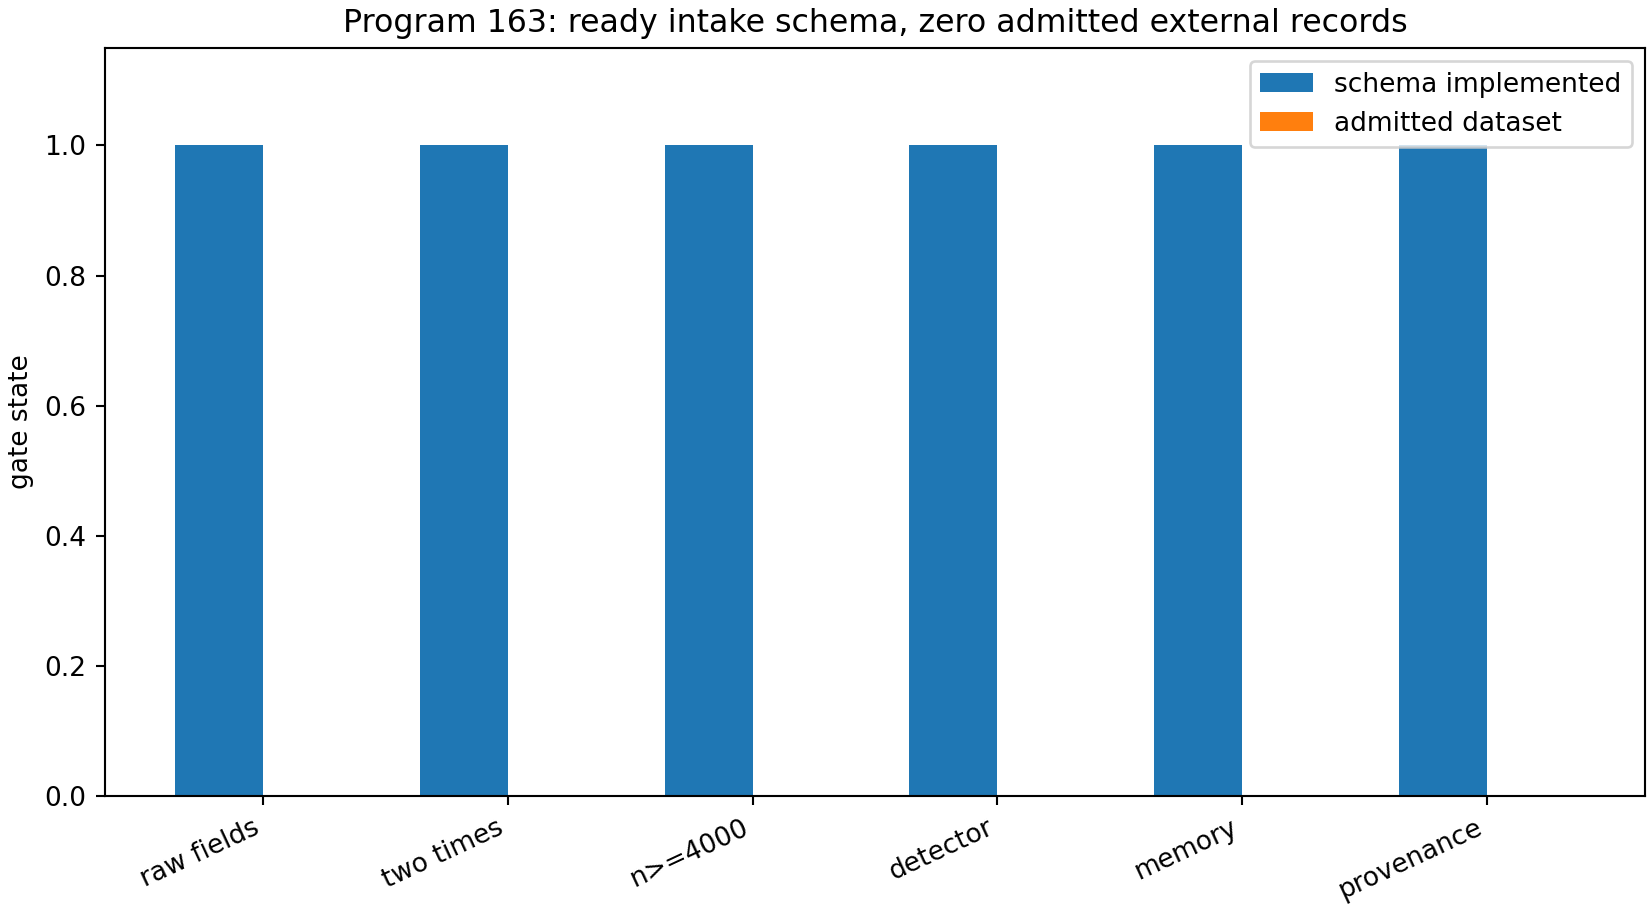
\includegraphics[width=0.94\textwidth]{FIN_Programs_151_164_Axiomatic_Operational_Figures/program163_external_readiness.png}
\caption{The intake schema is executable, while no external dataset is admitted.}
\end{figure}

\textbf{Result 163.1 [Proven for the local schema].} The validator and stop rules are executable. The explicit local intake directory contains zero candidates, so zero datasets are admitted.

No internet search or external download was made. This is readiness, not physical validation.

\par\medskip\hrule\medskip

\chapter{Program 164 --- AFIS: a minimal axiomatic architecture}

\section{Why axioms are now appropriate}

Earlier searches repeatedly tried to make one spectral object perform five logically different tasks. An axiomatic approach is useful because it asks a more precise question:

\begin{quote}\itshape
Which capability fails when a particular premise is removed?

\end{quote}

An axiom is admitted only if:

\begin{enumerate}
\item 
its mathematical type is explicit;

\item 
its output capability is explicit;

\item 
removing it has a countermodel;

\item 
it is not described as strict-derived;

\item 
it can, in principle, be replaced later by a source theorem.

\end{enumerate}

\section{Axiom A0 --- Conservative spectral Dirichlet generator}

\textbf{Statement.} There is a quadruple

\[
(\mathcal H,\mathcal E,A,\mathbf1)
\]

such that:

\begin{enumerate}
\item 
\(\mathcal E\) is a closed Markovian Dirichlet form;

\item 
\(A\) is its self-adjoint nonnegative generator;

\item 
\(A\mathbf1=0\).

\end{enumerate}

Then

\[
U_t=e^{-itA}
\]

is unitary and

\[
P_t=e^{-tA}
\]

is a positivity-preserving, conservative contraction semigroup.

The Green family is

\[
G_z=(A+zI)^{-1},\qquad z>0.
\]

\textbf{Necessity rank: 1 --- foundational.}

Each clause is needed:

\begin{itemize}
\item 
without self-adjointness, \(U_t\) need not be unitary and a projection-valued spectral measure is not guaranteed;

\item 
without nonnegativity, \(P_t\) can grow on negative spectrum;

\item 
without \(A\mathbf1=0\), total mass need not be conserved;

\item 
without the Markov property, a self-adjoint contraction need not preserve positivity.

\end{itemize}

This is the minimal object behind the shared wave/\allowbreak{}diffusion mathematics.

\section{Axiom A1 --- Sector equilibrium/\allowbreak{}state}

\textbf{Statement.} A localized finite algebra \(\mathcal A_F\) carries a faithful central state \(\omega_F\), and

\[
\eta=\omega_F(d).
\]

\(A_{\rm ME}\) from Program 154 is one explicit realization.

\textbf{Necessity rank: 3 --- model selection.}

\textbf{Countermodel on removal.} The uniform sector state and the normalized Hilbert-trace state share the same \(A_0\) but give

\[
\eta=\frac95
\quad\text{and}\quad
\eta=\frac{17}{9},
\]

respectively.

\section{Axiom A2 --- Preparation resource}

\textbf{Statement.} The theory declares an allowed set of preparation procedures. When an orientation-sensitive record is required, this set includes a nonfree signed resource \(M>0\).

\textbf{Necessity rank: 3 --- branch preparation.}

\textbf{Countermodel on removal.} Restrict all preparations to reflection-invariant states. Every reflection-odd receiver then has zero expectation under reflection-covariant processing.

A2 is not the observer. It is the mathematical interface describing how one state, among the kinematically possible states, is prepared.

\section{Axiom A3 --- Instrument, environment, apparatus, and record}

\textbf{Statement.} There is:

\begin{enumerate}
\item 
a normalized completely positive instrument \(\{\mathcal I_y\}\);

\item 
an apparatus/\allowbreak{}environment channel;

\item 
an outcome sigma-algebra;

\item 
a persistent record map.

\end{enumerate}

For initial state \(\rho\),

\[
\Pr(Y\in B)
=
\operatorname{Tr}
\left[
\int_B\mathcal I_y(\rho)\,dy
\right].
\]

\textbf{Necessity rank: 2 --- operational.}

\textbf{Countermodel on removal.} A state and its evolution may be fully defined while no map from the state to recorded outcomes exists. In that model no experimental probability has been defined.

This axiom contains the missing operational structure named in the preceding research: state, dynamics, clock interface, preparation, instrument, environment, apparatus and record are related but not conflated.

\section{Axiom A4 --- Dimensional calibration}

\textbf{Statement.} Every dimensional claim is accompanied by positive conversion standards and calibration maps. A minimal general package may be represented by

\[
(\ell_*,\tau_*,\hbar_*).
\]

\textbf{Necessity rank: 2 --- physical dimensions.}

\textbf{Countermodel on removal.} Rescale

\[
\ell_*\mapsto a\ell_*,
\qquad
\tau_*\mapsto b\tau_*,
\qquad
\hbar_*\mapsto c\hbar_*,
\]

while holding every dimensionless spectral identity fixed. Absolute length, time, energy and action change. No dimensionless theorem can distinguish the rescaled models.

A4 is the smallest missing bridge from dimensionless information to dimensionful measurement. It is not produced by Shannon entropy alone.

\section{Axiom A5 --- Typed legacy-to-strict completion}

\textbf{Statement.} There is a typed completion morphism carrying:

\begin{itemize}
\item 
amplitude;

\item 
damping and nonlinear compression;

\item 
phase and frequency;

\item 
selector/\allowbreak{}topological data;

\item 
an explicit role-semantics audit.

\end{itemize}

\textbf{Necessity rank: 4 --- FIN-specific completion.}

\textbf{Countermodel on removal.} The canonical legacy and strict kernels retain the nonzero scalar-completion residual and the phase representation obstruction of Program 160.

A5 does not assert that the bridge already exists. It specifies the exact object that a conditional full FIN model must supply.

\section{Capability theorem}

All 64 subsets of \(\{A_0,\ldots,A_5\}\) were enumerated.

\textbf{Theorem 164.1 \statusProven{}.} The unique minimum axiom sets for the declared capabilities are:

\begin{center}
\begingroup\small
\setlength{\tabcolsep}{3.5pt}
\renewcommand{\arraystretch}{1.16}
\begin{longtable}{@{}p{0.420\textwidth}p{0.420\textwidth}@{}}
\toprule
\textbf{capability} & \textbf{minimum axioms} \\
\midrule
\endhead
dual unitary/\allowbreak{}diffusive dynamics & \(\{A_0\}\) \\
target exponent as selected state & \(\{A_0,A_1\}\) \\
generic outcome probabilities & \(\{A_0,A_1,A_3\}\) \\
signed operational outcome & \(\{A_0,A_1,A_2,A_3\}\) \\
calibrated dimensional observation & \(\{A_0,A_1,A_3,A_4\}\) \\
calibrated signed test & \(\{A_0,A_1,A_2,A_3,A_4\}\) \\
typed kernel completion & \(\{A_0,A_1,A_5\}\) \\
eligibility for full role audit & \(\{A_0,\ldots,A_5\}\) \\
\bottomrule
\end{longtable}
\endgroup
\end{center}

\begin{figure}[htbp]
\centering
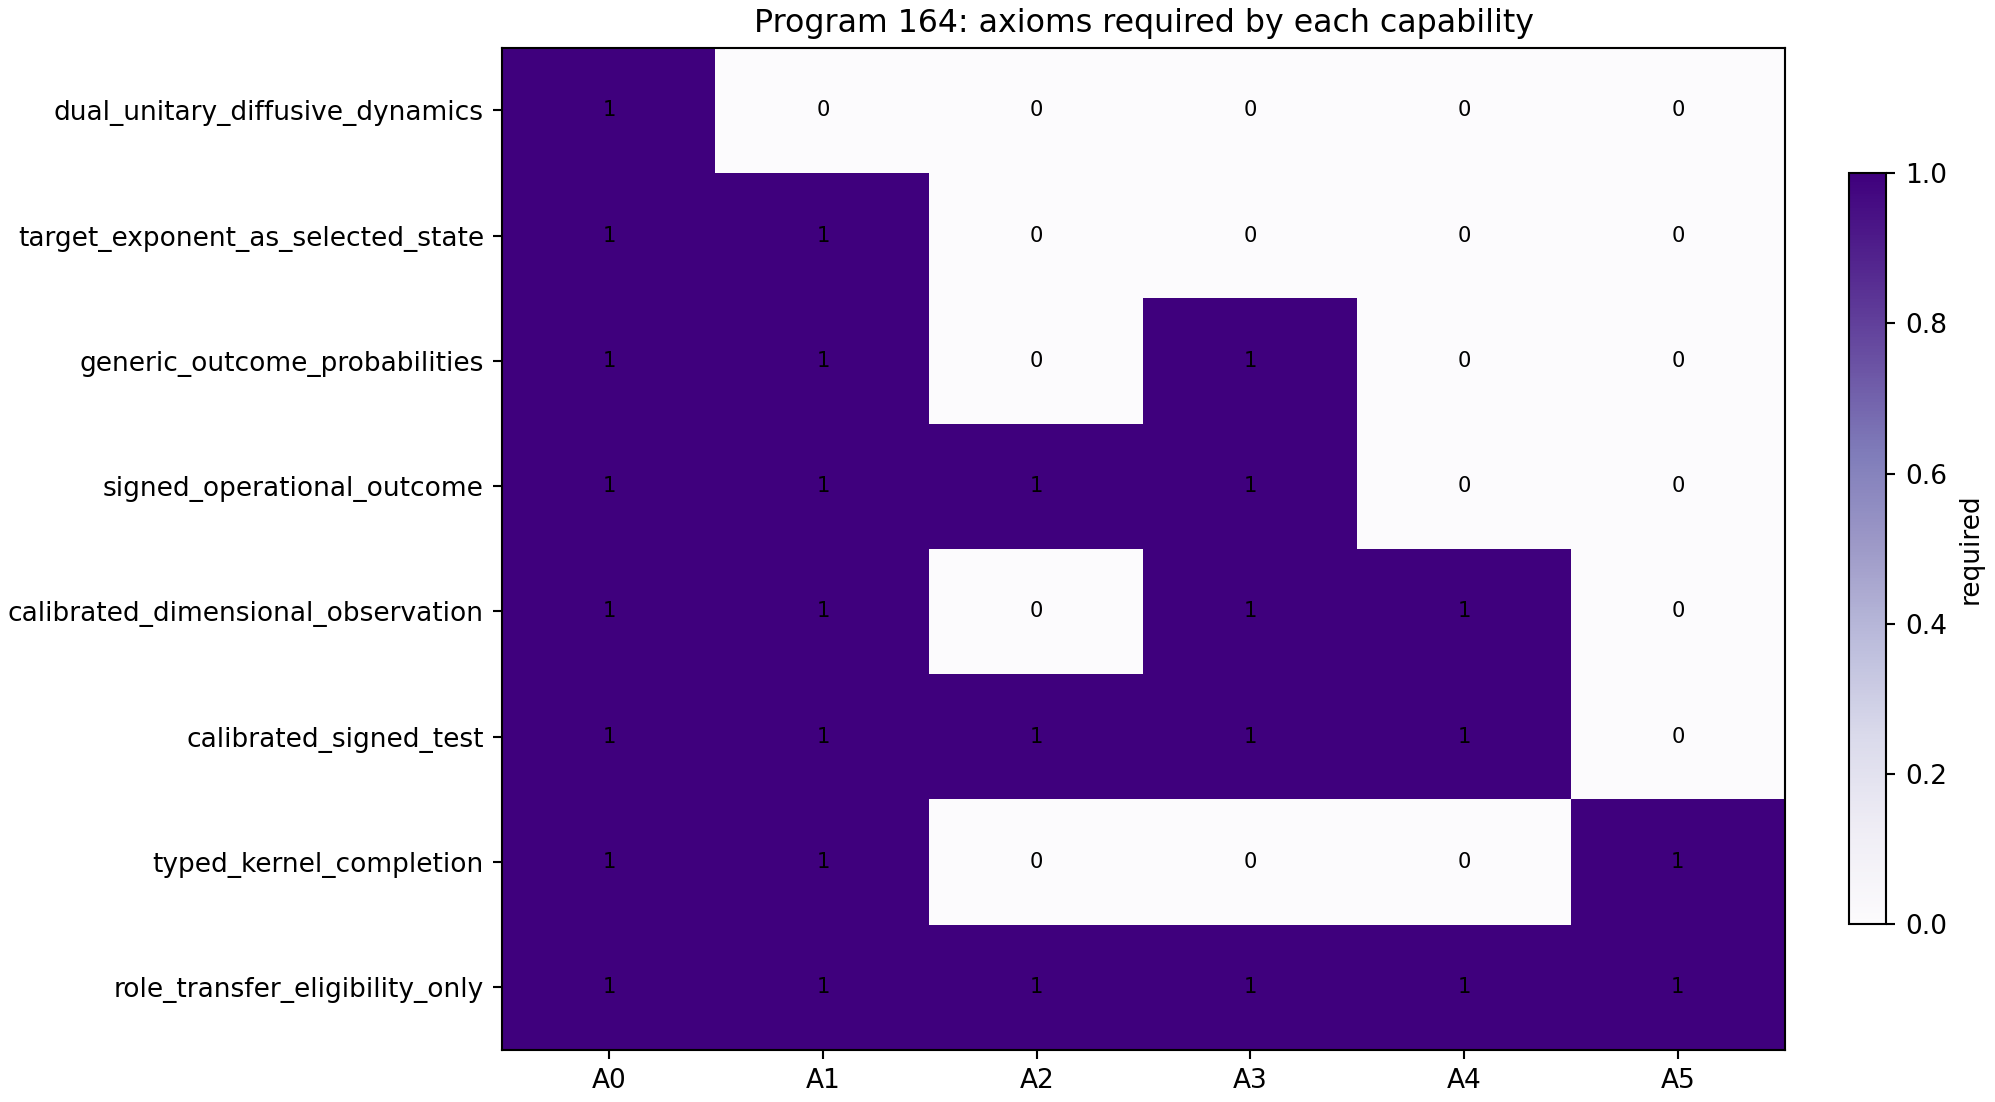
\includegraphics[width=0.94\textwidth]{FIN_Programs_151_164_Axiomatic_Operational_Figures/program164_axiom_capability_matrix.png}
\caption{Dependency of each mathematical or physical capability on the six AFIS axioms.}
\end{figure}

\section{Independence theorem}

\textbf{Theorem 164.2 \statusProven{}.} No one of \(A_1,\ldots,A_5\) follows from \(A_0\).

\textbf{Proof.} Fix one conservative spectral Dirichlet generator.

\begin{enumerate}
\item 
Choose two different faithful central states: A1 varies.

\item 
Choose a symmetric-only or signed preparation set: A2 varies.

\item 
Choose two different instruments, or no instrument: A3 varies.

\item 
Rescale the conversion standards: A4 varies.

\item 
Choose no legacy-to-strict completion or a declared conditional completion: A5 varies.

\end{enumerate}

All choices preserve the identical \(A_0\). Therefore none is a function of \(A_0\) without extra naturality assumptions. \(\square\)

\textbf{Corollary 164.3 \statusProven{}.} A theorem with input only the bare generator cannot uniquely output the selected state, signed preparation, instrument, physical unit system, and FIN-specific completion map.

This is the obstruction to a single universal "missing theorem".

\section{Smallest useful axiomatic branches}

The architecture should not always deploy all six axioms.

\subsection{Branch M --- spectral mathematics}

\[
\{A_0\}.
\]

This branch contains the spectral theorem, dual dynamics and Green family. It is the strictest mathematical core.

\subsection{Branch S --- selected dimensionless model}

\[
\{A_0,A_1\}.
\]

With \(A_{\rm ME}\), it yields \(\eta=9/5\) conditionally.

\subsection{Branch O --- generic operational physics}

\[
\{A_0,A_1,A_3\}.
\]

This branch defines outcome probabilities but need not produce a signed orientation.

\subsection{Branch SO --- signed operational physics}

\[
\{A_0,A_1,A_2,A_3\}.
\]

This branch supports orientation-sensitive preparations and records.

\subsection{Branch P --- calibrated signed test}

\[
\{A_0,A_1,A_2,A_3,A_4\}.
\]

This is the smallest branch able to compare a signed, dimensional prediction with a calibrated experiment.

\subsection{Branch F --- full conditional FIN}

\[
\{A_0,A_1,A_2,A_3,A_4,A_5\}.
\]

This branch is eligible to begin a role-transfer audit. Eligibility is not proof that any legacy physical role survives.

\par\medskip\hrule\medskip

\chapter{Cross-program falsification synthesis}

\section{Is one deeper object enough?}

There is one deeper object for the operator constructions:

\[
\boxed{
\text{conservative spectral Dirichlet generator}
}
\]

It unifies:

\begin{itemize}
\item 
the spectral measure;

\item 
wave evolution;

\item 
diffusion;

\item 
the Green family;

\item 
Dirichlet energy;

\item 
graph dynamics.

\end{itemize}

But it does not determine:

\begin{itemize}
\item 
which state is physically realized;

\item 
which sign or branch is prepared;

\item 
which measurement is performed;

\item 
which dimensional scale is used;

\item 
how legacy phase and damping complete to strict phase and compression;

\item 
which physical interpretation is attached to a record.

\end{itemize}

The correct conclusion is therefore neither "everything is independent" nor "everything is one shadow". The repository contains a single operator core surrounded by independent operational and conversion layers.

\section{Does the mirror coupling solve the selector?}

The reflection resource theory gives a precise answer.

A mirror/\allowbreak{}reflection operation introduces a \(\mathbb Z_2\) action. If the generator, state, preparation and instrument are all reflection-covariant, then a reflection-odd expectation remains zero. The symmetry is represented, not broken.

To break the symmetry one must add one of:

\begin{enumerate}
\item 
a signed preparation resource \(M>0\);

\item 
a noncovariant instrument;

\item 
a nonzero inversion-odd source coupled to the orientation torsor;

\item 
an explicit boundary or initial condition selecting a branch.

\end{enumerate}

Thus a mirror term can host the missing sign, but a symmetric mirror pair does not select its own polarity. It corresponds to a missing theoretical object only when its signed coupling or preparation is independently specified.

\section{Can information generate units?}

Shannon information and \(\alpha_{\rm geo}=4\log2\) are dimensionless. Any map

\[
H\longmapsto S_{\rm phys}
\]

requires a dimensionful conversion such as

\[
S_{\rm phys}=k_*H.
\]

Similarly, a phase weight needs

\[
e^{iS_{\rm phys}/\hbar_*}.
\]

The scale-rescaling countermodel proves that \(k_*\) and \(\hbar_*\) cannot be uniquely recovered from dimensionless spectral identities alone. They may be axioms, measured constants, or outputs of a future scale-charged source theorem. At present they are not strict outputs.

\section{The "observer paradox"}

The same generator supports

\[
U_t=e^{-itA}
\]

and

\[
P_t=e^{-tA}.
\]

There is no mathematical contradiction: both are Borel functions of \(A\). The apparent observer paradox begins only when one identifies one semigroup with unobserved evolution and the other with observed reduction without specifying an instrument.

A3 resolves the type error. The instrument, not \(P_t\) alone, maps a state to outcomes and post-measurement states. Diffusion may describe an environment, coarse graining, imaginary-time propagation, or a classical stochastic channel, but no one interpretation follows from functional calculus.

\par\medskip\hrule\medskip

\chapter{Final theorem and final answer}

\section{Axiomatic obstruction theorem}

\textbf{Theorem 17.1 \statusProven{}.} Within the category whose only input is a conservative spectral Dirichlet generator, no unique construction can simultaneously produce:

\begin{enumerate}
\item 
the target sector state;

\item 
a nonzero signed preparation;

\item 
an experimental instrument and record;

\item 
absolute physical dimensions;

\item 
a legacy-to-strict phase/\allowbreak{}compression completion.

\end{enumerate}

\textbf{Proof.} The countermodels of Theorem 164.2 keep the input object fixed and vary each requested output independently. A unique construction from the input would have to assign the same output to all models with that input, contradicting at least one variation. \(\square\)

The obstruction is simultaneously:

\begin{itemize}
\item 
\textbf{state-theoretic} for the sector state;

\item 
\textbf{resource-theoretic} for the signed preparation;

\item 
\textbf{operational} for the instrument and record;

\item 
\textbf{dimensional} for physical scales;

\item 
\textbf{representation-theoretic} for the phase completion.

\end{itemize}

It is not merely algebraic.

\section{Deepest surviving interpretation}

After the attempted constructions and falsifications, the deepest interpretation is:

\begin{quote}\itshape
FIN is most coherently formulated as an axiomatic informational-spectral operational theory. Its strict mathematical core is a conservative spectral Dirichlet generator associated with the informational nadsoliton. The generator unifies Green response, graph energy, unitary propagation and diffusive propagation. A physical theory arises only after independent state, preparation, instrument and calibration structures are supplied. The legacy-to-strict completion is a further FIN-specific obligation. No current theorem collapses these layers into one unavoidable object.

\end{quote}

The most promising new axiom is \(A_{\rm ME}\) because it closes one clearly identified problem with one equation and has a uniqueness proof. Its proper status is \textbf{conditional}, and that status is a scientific strength rather than a defect: the premise can now be attacked directly.

\par\medskip\hrule\medskip

\chapter{Recommended Programs 165--177}

The next studies should test the axioms instead of adding them silently.

\section{Program 165 --- Arb-certified oscillatory tail splitting}

Replace absolute tail domination by residue-class or Fourier-mode cancellation, use Arb/\allowbreak{}acb ball arithmetic, and certify the full \([10^{-3},2\cdot10^{-2}]\) window.

\textbf{Probability of a materially tighter theorem:} 0.80.\\
\textbf{Probability of a sub-\(3\%\) theorem with local resources:} 0.45.

\section{\texorpdfstring{Program 166 --- Derive or falsify \(A_{\rm ME}\) compositionally}{Program 166 --- Derive or falsify A\_ ME compositionally}}

Ask whether tensor additivity, independent composition of fibre systems, real-character functoriality, and stability under coarse graining force

\[
\beta_F=\alpha_{\rm geo}/4.
\]

Construct counterexamples before seeking uniqueness.

\textbf{Probability of a useful classification/\allowbreak{}no-go:} 0.85.\\
\textbf{Probability of strict derivation:} 0.20.

\section{Program 167 --- Formal AFIS consistency and independence}

Encode the finite-dimensional AFIS model and all removal countermodels in Lean, Isabelle, or another proof assistant. Separate analytic Dirichlet-form assumptions from finite matrix witnesses.

\textbf{Probability of formal completion:} 0.80.

\section{Program 168 --- Effective all-scale irrationality measure}

Search for an explicit theorem strong enough to establish \(D(\kappa,\nu)\) for \(743/(4000\pi)\), then propagate its actual constants into the Abelian remainder. Stop if constants are mathematically valid but numerically useless.

\textbf{Probability of some effective bound:} 0.55.\\
\textbf{Probability of a useful practical constant:} 0.15.

\section{Program 169 --- Monoidal groupoid valuation theorem}

Extend Program 153 from invariance to tensor products, induction, restriction, and valuation additivity. Classify all compatible orbit masses.

\textbf{Probability of classification:} 0.80.\\
\textbf{Probability of uniquely selecting uniform sector mass:} 0.25.

\section{\texorpdfstring{Program 170 --- Stability of the \(A_{\rm ME}\) equilibrium}{Program 170 --- Stability of the A\_ ME equilibrium}}

Perturb dimensions, energy gaps, degeneracies and \(\beta_F\). Derive the condition number of \(\eta\) and determine whether \(9/5\) is structurally stable or fine-tuned.

\textbf{Probability of a complete perturbation theorem:} 0.95.

\section{Program 171 --- Full reflection-resource theory}

Use semidefinite programming and representation theory to classify reflection-covariant channels on the full density space. Determine whether a finite family of monotones replaces \(M\).

\textbf{Probability of strong finite results:} 0.85.

\section{Program 172 --- Nonasymptotic detector statistics}

Add correlated noise, pixelization, censoring, estimated detector response and finite-memory channels. Derive honest bootstrap or concentration intervals and compare IQR with empirical characteristic-function estimators.

\textbf{Probability of an operationally useful procedure:} 0.85.

\section{Program 173 --- Calibration-control experimental design}

Construct the smallest set of known-input controls that makes the exponent score transverse to the apparatus tangent space. Optimize measurement times and allocation under a fixed record budget.

\textbf{Probability of an identifiability theorem:} 0.90.

\section{Program 174 --- Composite adversarial preregistration}

Replace the binary Program-150 rule with a preregistered comparison among Gaussian, stable, tempered, truncated, correlated, and gain-confounded families. Include model checking and abstention.

\textbf{Probability of reducing false FIN attribution:} 0.95.

\section{Program 175 --- General categorical phase obstruction}

Classify all equivariant maps among the legacy \(\mathbb Z_8\) character, the \(\mathbb Z_{12}\) carrier and the strict infinite-order phase. Quantify the minimal symmetry-breaking data required by a nonlinear completion.

\textbf{Probability of a general obstruction theorem:} 0.85.

\section{Program 176 --- One explicit nonlinear completion candidate}

Construct exactly one typed nonlinear map with independent amplitude, compression and phase-source slots. Audit it against the six Program-162 edges. Stop at the first failed edge.

\textbf{Probability of a useful obstruction:} 0.80.\\
\textbf{Probability of complete positive bridge:} 0.10.

\section{Program 177 --- AFIS measurement model for double-slit records}

Build a finite CP-instrument model with preparation, propagation, environmental decoherence, detector resolution and persistent record. Demonstrate exactly which interference and which diffusion statements follow from \(A_0\)--\(A_4\), without attributing collapse to \(P_t\) alone.

\textbf{Probability of a rigorous conditional model:} 0.90.\\
\textbf{Probability of strict physical validation without data:} 0.

\section{Priority}

The recommended order is

\[
166\to170\to167\to173\to174\to172\to165
\to171\to175\to177\to169\to168\to176.
\]

The priority is intentionally axiom-first:

\begin{enumerate}
\item 
try to derive or falsify the most economical new axiom;

\item 
quantify its stability;

\item 
formalize independence;

\item 
repair experimental identifiability;

\item 
return to the expensive bridge only with a typed candidate.

\end{enumerate}

\par\medskip\hrule\medskip

\chapter{Reproducibility statement}

The executable research file is:

fin\_programs\_151\_164\_axiomatic\_operational\_foundations.py

The machine-readable results are:

FIN\_Programs\_151\_164\_Axiomatic\_Operational\_Results.json

The extracted axiom system is:

FIN\_Programs\_151\_164\_Minimal\_Axiomatic\_System.json

Regression tests are:

test\_fin\_programs\_151\_164\_axiomatic\_operational\_foundations.py

Fourteen figures are generated in:

FIN\_Programs\_151\_164\_Axiomatic\_Operational\_Figures/\allowbreak{}

The study uses no external physical data.

\par\medskip\hrule\medskip

\chapter{Selected references}

\begin{enumerate}
\item 
M. Reed and B. Simon, \emph{Methods of Modern Mathematical Physics I: Functional Analysis}, Academic Press.

\item 
E. B. Davies, \emph{Heat Kernels and Spectral Theory}, Cambridge University Press.

\item 
M. Fukushima, Y. Oshima and M. Takeda, \emph{Dirichlet Forms and Symmetric Markov Processes}, de Gruyter.

\item 
O. Bratteli and D. W. Robinson, \emph{Operator Algebras and Quantum Statistical Mechanics}, Springer.

\item 
M. Takesaki, \emph{Theory of Operator Algebras I}, Springer.

\item 
L. Kuipers and H. Niederreiter, \emph{Uniform Distribution of Sequences}, Wiley.

\item 
K. Sato, \emph{Lévy Processes and Infinitely Divisible Distributions}, Cambridge University Press.

\item 
A. W. van der Vaart, \emph{Asymptotic Statistics}, Cambridge University Press.

\item 
A. S. Holevo, \emph{Probabilistic and Statistical Aspects of Quantum Theory}, North-Holland.

\item 
E. B. Davies and J. T. Lewis, "An operational approach to quantum probability," \emph{Communications in Mathematical Physics} 17 (1970).

\item 
F. G. Brandão and G. Gour, "Reversible framework for quantum resource theories," \emph{Physical Review Letters} 115 (2015).

\item 
S. Mac Lane, \emph{Categories for the Working Mathematician}, Springer.

\end{enumerate}

\par\medskip\hrule\medskip

\chapter{Suggested citation}

\.Zuchowski, K. (2026). \emph{FIN Programs 151--164: Axiomatic Operational Foundations, State Selection, and Falsifiable Measurement} (FIN Research Monograph, Release 10.15; Version 1.0.0) [Preprint]. Zenodo.


\clearpage
\chapter*{Archival note}
\addcontentsline{toc}{chapter}{Archival note}
Machine-readable results are stored in
\path{FIN_Programs_151_164_Axiomatic_Operational_Results.json}.
The extracted six-axiom system is stored in
\path{FIN_Programs_151_164_Minimal_Axiomatic_System.json}.
The executable, sixty-two tests, and fourteen figures reproduce the release.

\medskip
\noindent\textbf{Suggested citation:}

\.Zuchowski, K. (2026). \emph{FIN Programs 151--164: Axiomatic Operational
Foundations, State Selection, and Falsifiable Measurement}
(FIN Research Monograph, Release 10.15; Version 1.0.0) [Preprint]. Zenodo.
\end{document}
